\documentclass{beamer}

\mode<presentation> {
	\usetheme{Boadilla}
	%\usetheme{CambridgeUS}
}
\usefonttheme[onlymath]{serif}
\usepackage{graphicx}
\usepackage{booktabs} % Allows the use of \toprule, \midrule and \bottomrule in tables
\usepackage{amssymb,mathrsfs,amsmath}
\usepackage{bbding}
\usepackage{amsfonts}
\usepackage{enumerate}
\usepackage{color}
\usepackage{xcolor}
%-------------------------------------------------------------------------

\title[Am. Econ. Rev. 2018]{Commuting, Migration, and Local Employment Elasticities}
\author[Monte, Redding \& Rossi-Hansberg]{Ferdinando Monte, Stephen J. Redding, and Esteban Rossi-Hansberg} 
\institute[]{Presenter: Qinzhu Sun}

\date{\today}
\logo{
\includegraphics[scale=0.2]{maingate2}}
\begin{document}

\begin{frame}
	\titlepage
\end{frame}

\begin{frame}{Overview}
	\tableofcontents
\end{frame}
%-------------------------------------------------------------------------
%-------------------------------------------------------------------------
\section{Introduction}
\begin{frame}[shrink]
	\transfade %fade in and fade out
	\tableofcontents[sectionstyle=show/shaded,subsectionstyle=show/shaded/hide]
	\addtocounter{framenumber}{-1}
\end{frame}
%------------------------------------------------
\begin{frame}{Introduction}
	The ability of firms to attract workers depends on the ability to attract
	\begin{itemize}
		\item local residents through migration,
		\item and commuters from other nearby locations.
	\end{itemize}
	\medskip

	$\Rightarrow$ Together, \textcolor{red}{migration} and \textcolor{red}{commuting} determine the response of local employment to local labor demand shocks (local employment elasticity).
\end{frame}
%------------------------------------------------
\begin{frame}{The prevalence of commuting}
	\begin{figure}[htbp]
		\centering
		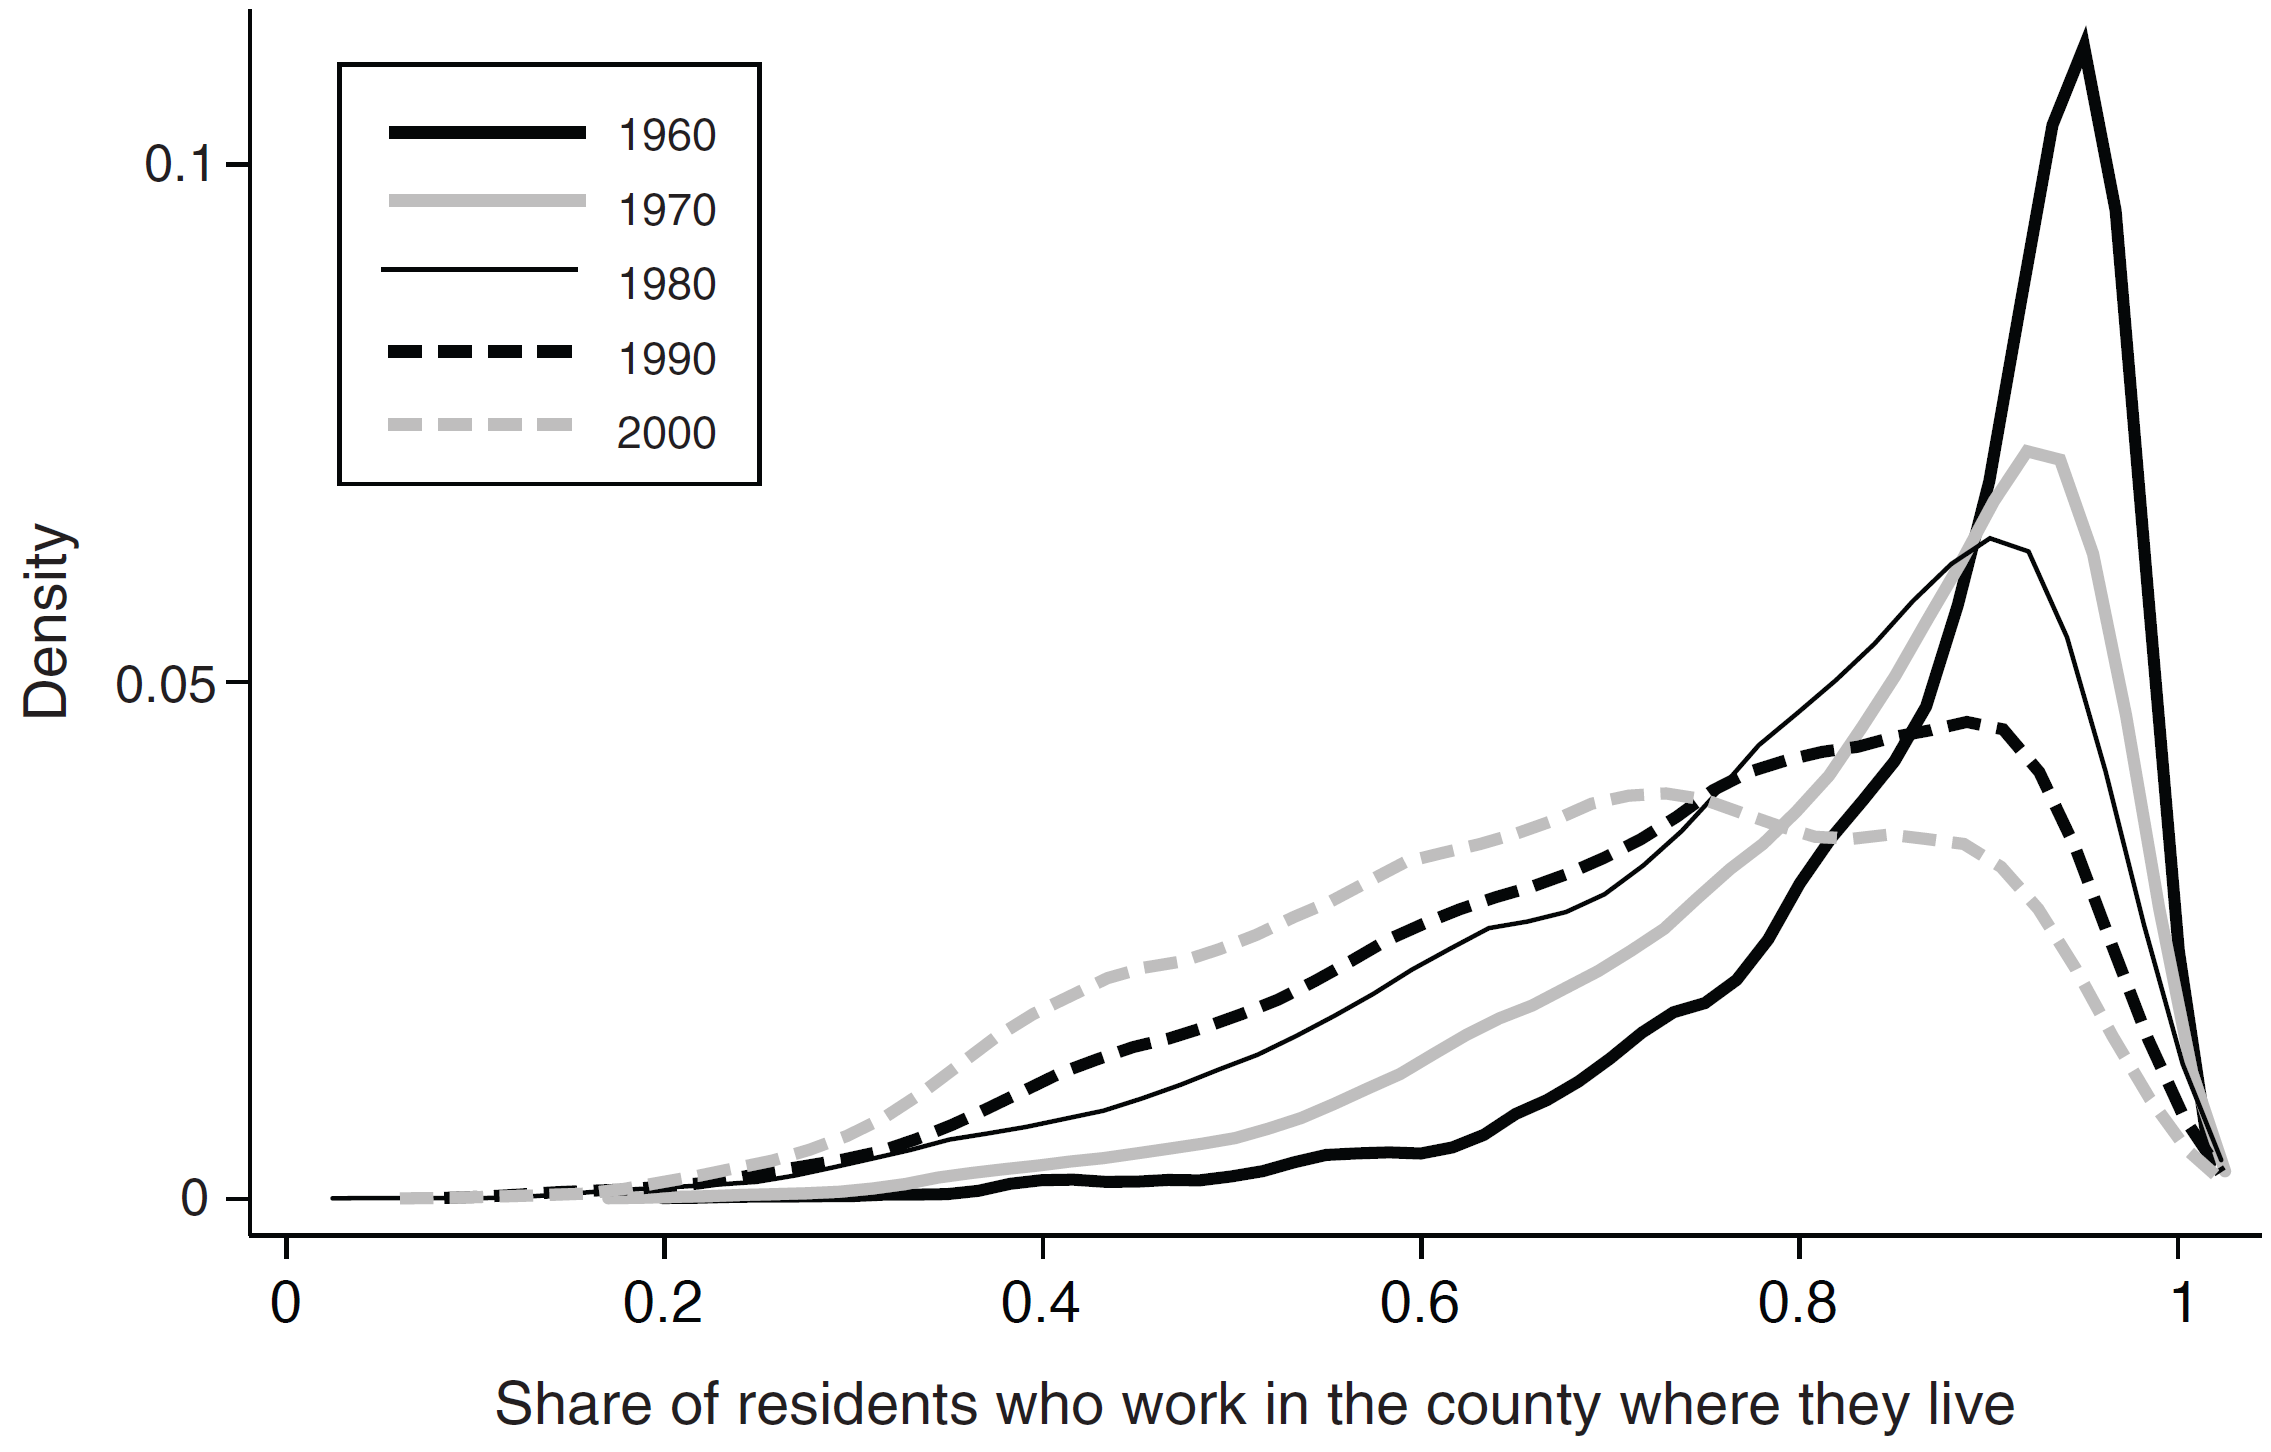
\includegraphics[width=0.9\textwidth]{fig1.png}
	\end{figure}
\end{frame}
%------------------------------------------------
\begin{frame}{What this paper does}
	\textbf{1.} Develop \textcolor{red}{a quantitative GE model} with spatial linkages in both goods markets and factor markets.
	\begin{itemize}
		\item The local employment elasticity is \textcolor{red}{endogenous} and differs, depending on their linkages to one another.
		\item A large part of the variation results from differences in commuting links between a location and its neighbors.
	\end{itemize}
	\medskip

	\textbf{2.} Provide \textcolor{red}{empirical evidence} for the importance of commuting for employment changes using the quasi-experiment of MDP.\footnote{\textit{"Million Dollar Plant"} following Greenstone, Hornbeck \& Moretti (2010) (GHM)}
	\begin{itemize}
		\item \textbf{Finding:} Greater increases in employment from the positive labor demand shock in counties with more open commuting markets.
	\end{itemize}
	\medskip

	\textbf{3.} Evaluate the \textcolor{red}{counterfactual} effects of changes in trade and commuting costs. (Head \& Ries (2001); DEK (2008))
\end{frame}
%------------------------------------------------
\begin{frame}{Literature review}
	\textbf{International trade}
	\begin{itemize}
		\item Quantitative models of costly trade in goods since EK (2002).
	\end{itemize}
	\medskip

	\textbf{Economic geography}
	\begin{itemize}
		\item Costly trade in goods and factor mobility, with \textit{variation across regions or systems of cities}.
		\item {\small Krugman (1991); FKV (1999); Redding \& Sturm (2008); Allen \& Arkolakis (2014); Desmet \& Rossi-Hansberg (2014); Redding (2016) \dots}
	\end{itemize}
	\medskip

	\textbf{Urban economics}
	\begin{itemize}
		\item Costly movement of people (commuting), with \textit{variation within cities}.
		\item {\small Alonso (1964); Mills (1967); Muth (1969); Lucas \& Rossi-Hansberg (2002); Desmet \& Rossi-Hansberg (2013); Ahlfeldt et al. (2015) \dots}
	\end{itemize}
\end{frame}
%------------------------------------------------
\begin{frame}{Literature review}
	\textbf{Local labor markets}
	\begin{itemize}
		\item Estimating the effects of local labor demand shocks, without the view of spatial linkages.
		\item Bartik (1991); GHM (2010); Autor, Dorn \& Hanson (2013) \dots
	\end{itemize}
\end{frame}
%------------------------------------------------
\begin{frame}{Contributions}
	\begin{block}{Spatial economy}
		\begin{itemize}
			\item Develop a tractable framework in which an arbitrary set of regions are linked in both goods markets and labor markets, with both within- and across-city interactions.
			\item Quantify with disaggregated data on trade and commuting for the US and conduct counterfactuals.
			\item Establish the importance of spatial interactions between locations in determining the effects of local labor demand shocks.
		\end{itemize}
	\end{block}
	\begin{block}{Local labor markets}
		\begin{itemize}
			\item Show that understanding the spatial linkages is central to evaluating the local impact of economic shocks.
		\end{itemize}
	\end{block}
\end{frame}
%-------------------------------------------------------------------------
%-------------------------------------------------------------------------
\section{Model}
\begin{frame}[shrink]
	\transfade %fade in and fade out
	\tableofcontents[sectionstyle=show/shaded,subsectionstyle=show/shaded/hide]
	\addtocounter{framenumber}{-1}
\end{frame}
%------------------------------------------------
\begin{frame}{Preference and endowments}
	The preference of a worker $\omega$ who lives and consumes in location $n$ and works in location $i$ is defined by
	\begin{equation}
		U_{ni\omega} = \frac{b_{ni\omega}}{\kappa_{ni}}\left(\frac{C_{n\omega}}{\alpha}\right)^\alpha \left(\frac{H_{n\omega}}{1-\alpha}\right)^{1-\alpha},
	\end{equation}
	where
	\begin{itemize}
		\item $b_{ni\omega}$ is an idiosyncratic amenities shock
		\item $\kappa_{ni}\in [1,\infty)$ is an iceberg commuting cost
		\item $C_{n\omega}$ is final goods consumption
		\item $H_{n\omega}$ is residential land use.
	\end{itemize}
\end{frame}
%------------------------------------------------
\begin{frame}{Preference and endowments}
	The idiosyncratic amenities $b_{ni\omega}$ are drawn from an independent Fr\'echet distribution
	\begin{equation}
		G_{ni}(b) = e^{-B_{ni}b^{-\epsilon}}, \quad B_{ni}>0,\; \epsilon > 1,
	\end{equation}
	where
	\begin{itemize}
		\item the scale parameter $B_{ni}$ determines the average amenities
		\item the shape parameter $\epsilon>1$  controls the dispersion of amenities.
	\end{itemize}
\end{frame}
%------------------------------------------------
\begin{frame}{Preference and endowments}
	The goods consumption index in location $n$ is a CES function of a continuum of tradable varieties from each location $i$,
	\begin{equation}
		C_n = \left[\sum_{i\in N}\int_0^{M_i}c_{ni}(j)^\rho dj \right]^{1/\rho},\quad \sigma=\frac{1}{1-\rho}>1.
	\end{equation}
	\textbf{Utility maximization} $\Rightarrow$
	\begin{equation}
		c_{ni}(j)=\alpha X_nP_n^{\sigma-1}p_{ni}(j)^{-\sigma},
	\end{equation}
	where
	\begin{itemize}
		\item $X_n$ is aggregate expenditure in location $n$
		\item $P_n=\left[\sum_{i\in N}\int_0^{M_i}p_{ni}(j)^{1-\sigma} dj\right]^{\frac{1}{1-\sigma}}$ is the price index
		\item $p_{ni}(j)$ is the price of a variety $j$ produced in $i$ and consumed in $n$.
	\end{itemize}
\end{frame}
%------------------------------------------------
\begin{frame}{Preference and endowments}
	\textbf{Utility maximization} $\Rightarrow$ A fraction $1-\alpha$ of worker income is spent on residential land.
	\medskip

	\textbf{Assumption:} Land is owned by immobile landlords, who receive worker expenditure on land as income, and consume only goods where they live.
	\begin{equation}
		P_nC_n = \alpha \bar{v}_nR_n + (1-\alpha)\bar{v}_nR_n = \bar{v}_nR_n,
	\end{equation}
	where
	\begin{itemize}
		\item $\bar{v}_n$ is the average labor income across employment locations
		\item $R_n$ is the measure of residents.
	\end{itemize}
	\medskip
	\textbf{Land market clearing condition}
	\begin{equation}
		Q_n = (1-\alpha)\frac{\bar{v}_nR_n}{H_n}.
	\end{equation}
\end{frame}
%------------------------------------------------
\begin{frame}{Production}
	Varieties are produced using labor under monopolistic competition and increasing returns to scale.
	\begin{equation}
		l_i(j) = F + x_i(j)/A_i.
	\end{equation}
	\textbf{Profit maximization} $\Rightarrow$
	\begin{equation}
		p_{ni}(j)=\left(\frac{\sigma}{\sigma-1} \right)\frac{d_{ni}w_i}{A_i}.
	\end{equation}
	\textbf{Profit maximization} + \textbf{Zero profit condition} $\Rightarrow$
	\begin{equation}
		x_i(j) = A_iF(\sigma-1).
	\end{equation}
	The total measure of produced varieties is
	\begin{equation}
		M_i=L_i/(\sigma F).
	\end{equation}
\end{frame}
%------------------------------------------------
\begin{frame}{Goods trade}
	The share of location $n$'s expenditure on goods produced in location $i$ is
	\begin{equation}
		\pi_{ni} = \frac{M_ip_{ni}^{1-\sigma}}{\sum_{k\in N}M_kp_{nk}^{1-\sigma}}=\frac{L_i(d_{ni}w_i/A_i)^{1-\sigma}}{\sum_{k\in N}L_k(d_{nk}w_k/A_k)^{1-\sigma}}.
	\end{equation}
	\textbf{Trade balance}
	\begin{equation}
		w_iL_i = \sum_{n\in N}\pi_{ni}\bar{v}_nR_n.
	\end{equation}
	The price index can be expressed as
	\begin{small}
		\begin{equation}
			\begin{aligned}
				P_n &= \left[\sum_{i\in N}\int_0^{M_i}p_{ni}(j)^{1-\sigma} dj\right]^{\frac{1}{1-\sigma}} \\
				&= \frac{\sigma}{\sigma-1}\left(\frac{1}{\sigma F}\right)^{\frac{1}{1-\sigma}}\left[\sum_{i\in N}L_i(d_{ni}w_i/A_i)^{1-\sigma} \right]^{\frac{1}{1-\sigma}} \\
				&= \frac{\sigma}{\sigma-1}\left(\frac{L_n}{\sigma F\pi_{nn}}\right)^{\frac{1}{1-\sigma}}\frac{d_{nn}w_n}{A_n}.
			\end{aligned}
		\end{equation}
	\end{small}
\end{frame}
%------------------------------------------------
\begin{frame}{Labor mobility and commuting}
	\textbf{Indirect utility}
	\begin{equation}
		U_{ni\omega} = \frac{b_{ni\omega}w_i}{\kappa_{ni}P_n^\alpha Q_n^{1-\alpha}}.
	\end{equation}
	\medskip

	$\Rightarrow$ The probability that a worker chooses to live in $n$ and work in $i$ is
	\begin{equation}
		\lambda_{ni} = \frac{B_{ni}\left(\kappa_{ni}P_n^\alpha Q_n^{1-\alpha}\right)^{-\epsilon}w_i^{\epsilon}}{\sum_{r\in N}\sum_{s\in N}B_{rs}\left(\kappa_{rs}P_r^\alpha Q_r^{1-\alpha}\right)^{-\epsilon}w_s^{\epsilon}}\equiv \frac{\Phi_{ni}}{\Phi}.
	\end{equation}
	$\Rightarrow$
	\begin{equation}
		\lambda_n^R = \frac{R_n}{\bar{L}}=\sum_{i\in N}\lambda_{ni}=\sum_{i\in N}\frac{\Phi_{ni}}{\Phi},\quad \lambda_i^L = \frac{L_i}{\bar{L}}=\sum_{n\in N}\lambda_{ni}=\sum_{n\in N}\frac{\Phi_{ni}}{\Phi}.
	\end{equation}
	\begin{block}{}
		Comparative statics: $(P_n, Q_n, w_i, \kappa_{ni}, B_{ni})$
	\end{block}
\end{frame}
%------------------------------------------------
\begin{frame}{Labor mobility and commuting}
	The probability that a worker commutes to $i$ conditional on living in $n$ is
	\begin{equation}
		\lambda_{ni|n}^R \equiv \frac{\lambda_{ni}}{\lambda_n^R} = \frac{B_{ni}(w_i/\kappa_{ni})^{\epsilon}}{\sum_{s\in N}B_{ns}(w_s/\kappa_{ns})^{\epsilon}}.
	\end{equation}
	\textbf{Labor market clearing condition}
	\begin{equation}
		L_i = \sum_{n\in N}\lambda_{ni|n}^R R_n.
	\end{equation}
	\textbf{Expected worker income}
	\begin{equation}
		\bar{v}_n = \sum_{i\in N}\lambda_{ni|n}^R w_i.
	\end{equation}
\end{frame}
%------------------------------------------------
\begin{frame}{Labor mobility and commuting}
	\textbf{Population mobility}
	\begin{equation}
		\begin{aligned}
			\bar{U} &= E\left[U_{ni\omega}\right] \\
			&= \Gamma\left(\frac{\epsilon-1}{\epsilon}\right)\left[ \sum_{r\in N}\sum_{s\in N}B_{rs}\left(\kappa_{rs}P_r^\alpha Q_r^{1-\alpha}\right)^{-\epsilon}w_s^\epsilon\right]^{1/\epsilon}, \quad \forall n,i \in N.
		\end{aligned}
	\end{equation}
\end{frame}
%------------------------------------------------
\begin{frame}{General equilibrium}
	The general equilibrium can be referenced by the following vector of six variables $\left\{w_n,\bar{v}_n, Q_n, L_n, R_n, P_n \right\}_{n=1}^N $ and a scalar $\bar{U}$.
	\small
	\begin{equation}\nonumber
		w_iL_i = \sum_{n\in N}\pi_{ni}\bar{v}_nR_n
	\end{equation}
	\begin{equation}\nonumber
		\bar{v}_n = \sum_{i\in N}\lambda_{ni|n}^R w_i
	\end{equation}
	\begin{equation}\nonumber
		Q_n = (1-\alpha)\frac{\bar{v}_nR_n}{H_n}
	\end{equation}
	\begin{equation}\nonumber
		\lambda_n^R = \frac{R_n}{\bar{L}}=\sum_{i\in N}\lambda_{ni}=\sum_{i\in N}\frac{\Phi_{ni}}{\Phi},\quad \lambda_i^L = \frac{L_i}{\bar{L}}=\sum_{n\in N}\lambda_{ni}=\sum_{n\in N}\frac{\Phi_{ni}}{\Phi}
	\end{equation}
	\begin{equation}\nonumber
		P_n = \frac{\sigma}{\sigma-1}\left(\frac{L_n}{\sigma F\pi_{nn}}\right)^{\frac{1}{1-\sigma}}\frac{d_{nn}w_n}{A_n}
	\end{equation}
	\begin{equation}\nonumber
		\bar{L} = \sum_{n\in N}R_n = \sum_{n\in N}L_n.
	\end{equation}
\end{frame}
%-------------------------------------------------------------------------
%-------------------------------------------------------------------------
\section{Data and Measurement}
\begin{frame}[shrink]
	\transfade %fade in and fade out
	\tableofcontents[sectionstyle=show/shaded,subsectionstyle=show/shaded/hide]
	\addtocounter{framenumber}{-1}
\end{frame}
%------------------------------------------------
\begin{frame}{Data and Measurement}
	\begin{table}[]
		\begin{tabular}{ll}
		\hline \hline
		Variables    & Source      \\ \hline
		Trade and distances & Commodity Flow Survey    \\
		Commuting      & American Community Survey 2006-2010, \\
		& US Census 1960-2000  \\ 
		Employment and wages     & Bureau of Economic Analysis \\ 
		\dots  & GIS     \\ \hline
		\end{tabular}
	\end{table}
\end{frame}
%------------------------------------------------
\begin{frame}{Data and Measurement}
	\textbf{Goods Trade}
	\begin{equation}
		\textcolor{red}{w_iL_i}-\sum_{n\in N} \frac{\textcolor{red}{L_i}(\textcolor{blue}{d_{ni}}\textcolor{red}{w_i}/A_i)^{1-\sigma}}{\sum_{k\in N}\textcolor{red}{L_k}(\textcolor{blue}{d_{nk}}\textcolor{red}{w_k}/A_k)^{1-\sigma}}[\textcolor{red}{\bar{v}R_n}+\textcolor{red}{D_n}] = 0,
	\end{equation}
	\textbf{Commuting Flows}
	\begin{equation}
		\textcolor{red}{\lambda_{ni}} = \frac{\mathcal{B}_{ni}\left(\frac{\textcolor{red}{L_n}}{\textcolor{red}{\pi_{nn}}}\right)^{-\frac{\alpha\epsilon}{\sigma-1}}A_n^{\alpha\epsilon}\textcolor{red}{w_n}^{-\alpha\epsilon}\textcolor{red}{\bar{v}_n}^{-\epsilon(1-\alpha)}\left(\frac{\textcolor{red}{R_n}}{\textcolor{red}{H_n}}\right)^{-\epsilon(1-\alpha)}\textcolor{red}{w_i}^{\epsilon}}
		{\sum_{r\in N}\sum_{s\in N}\mathcal{B}_{rs}\left(\frac{\textcolor{red}{L_r}}{\textcolor{red}{\pi_{rr}}}\right)^{-\frac{\alpha\epsilon}{\sigma-1}}A_r^{\alpha\epsilon}\textcolor{red}{w_r}^{-\alpha\epsilon}\textcolor{red}{\bar{v}_r}^{-\epsilon(1-\alpha)}\left(\frac{\textcolor{red}{R_r}}{\textcolor{red}{H_r}}\right)^{-\epsilon(1-\alpha)}\textcolor{red}{w_s}^{\epsilon}},
	\end{equation}
	where $\mathcal{B}_{ni}\equiv B_{ni}\kappa_{ni}^{-\epsilon}$ captures the ease of commuting.
\end{frame}
%------------------------------------------------
\begin{frame}{Data and Measurement}
	\begin{figure}[htbp]
		\centering
		Commuting across Counties and Commuting Zones (Unweighted)
		\medskip

		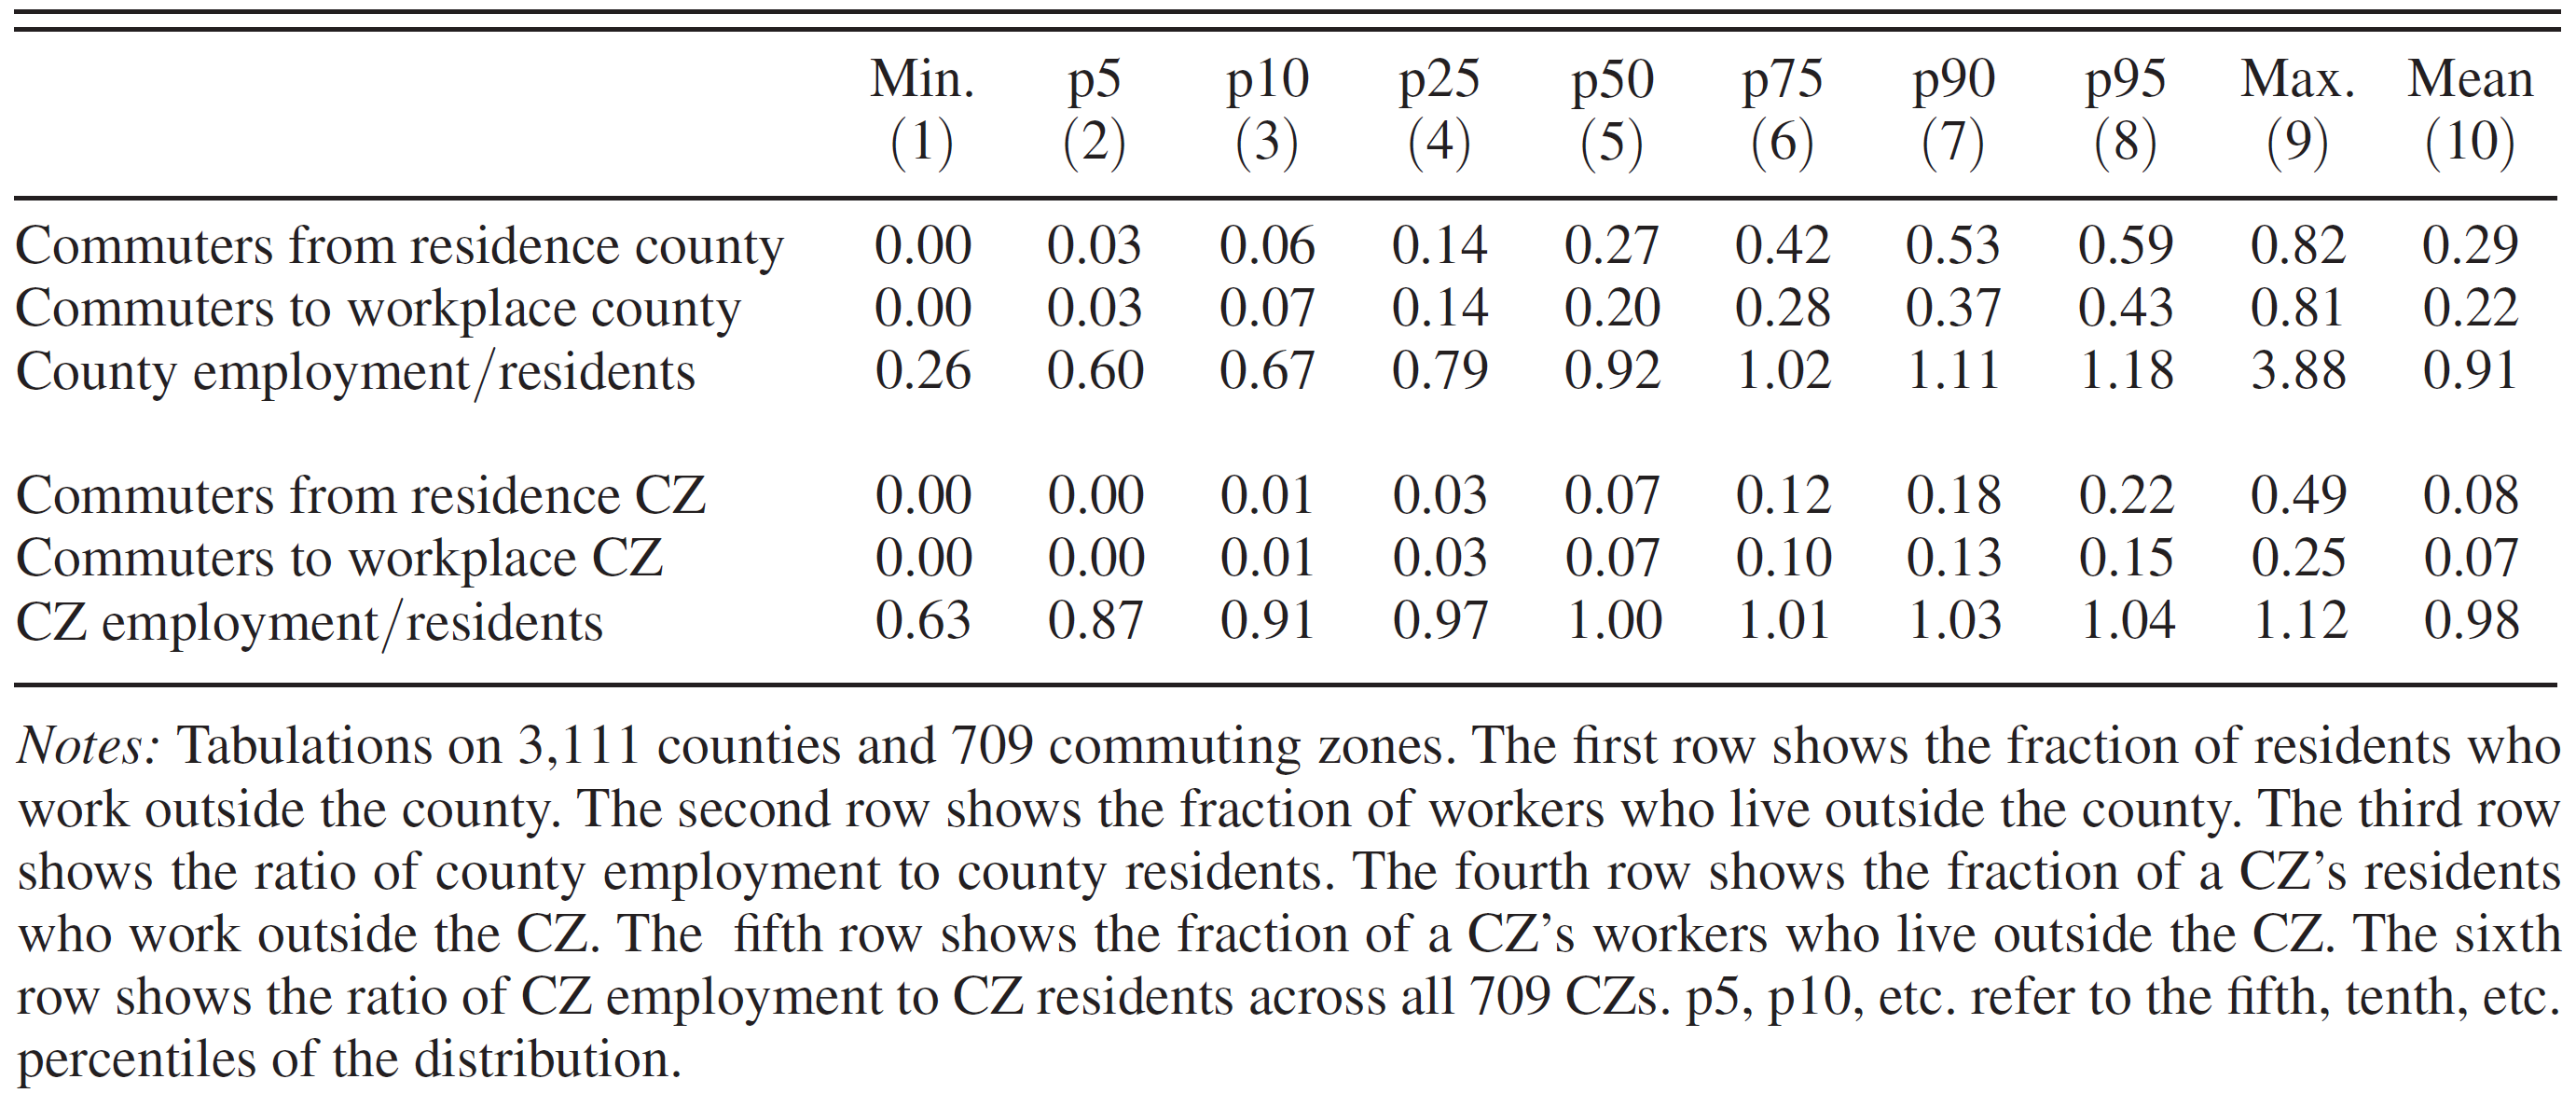
\includegraphics[width=0.9\textwidth]{tab1.png}
	\end{figure}
\end{frame}
%-------------------------------------------------------------------------
%-------------------------------------------------------------------------
\section{Local Employment Elasticities}
\begin{frame}[shrink]
	\transfade %fade in and fade out
	\tableofcontents[sectionstyle=show/shaded,subsectionstyle=show/shaded/hide]
	\addtocounter{framenumber}{-1}
\end{frame}
%------------------------------------------------
\begin{frame}{Elasticity heterogeneity}
	We compute 3111 counterfactual exercises, imposing each county with a 5\% productivity shock.
	\begin{figure}[htbp]
		\centering
		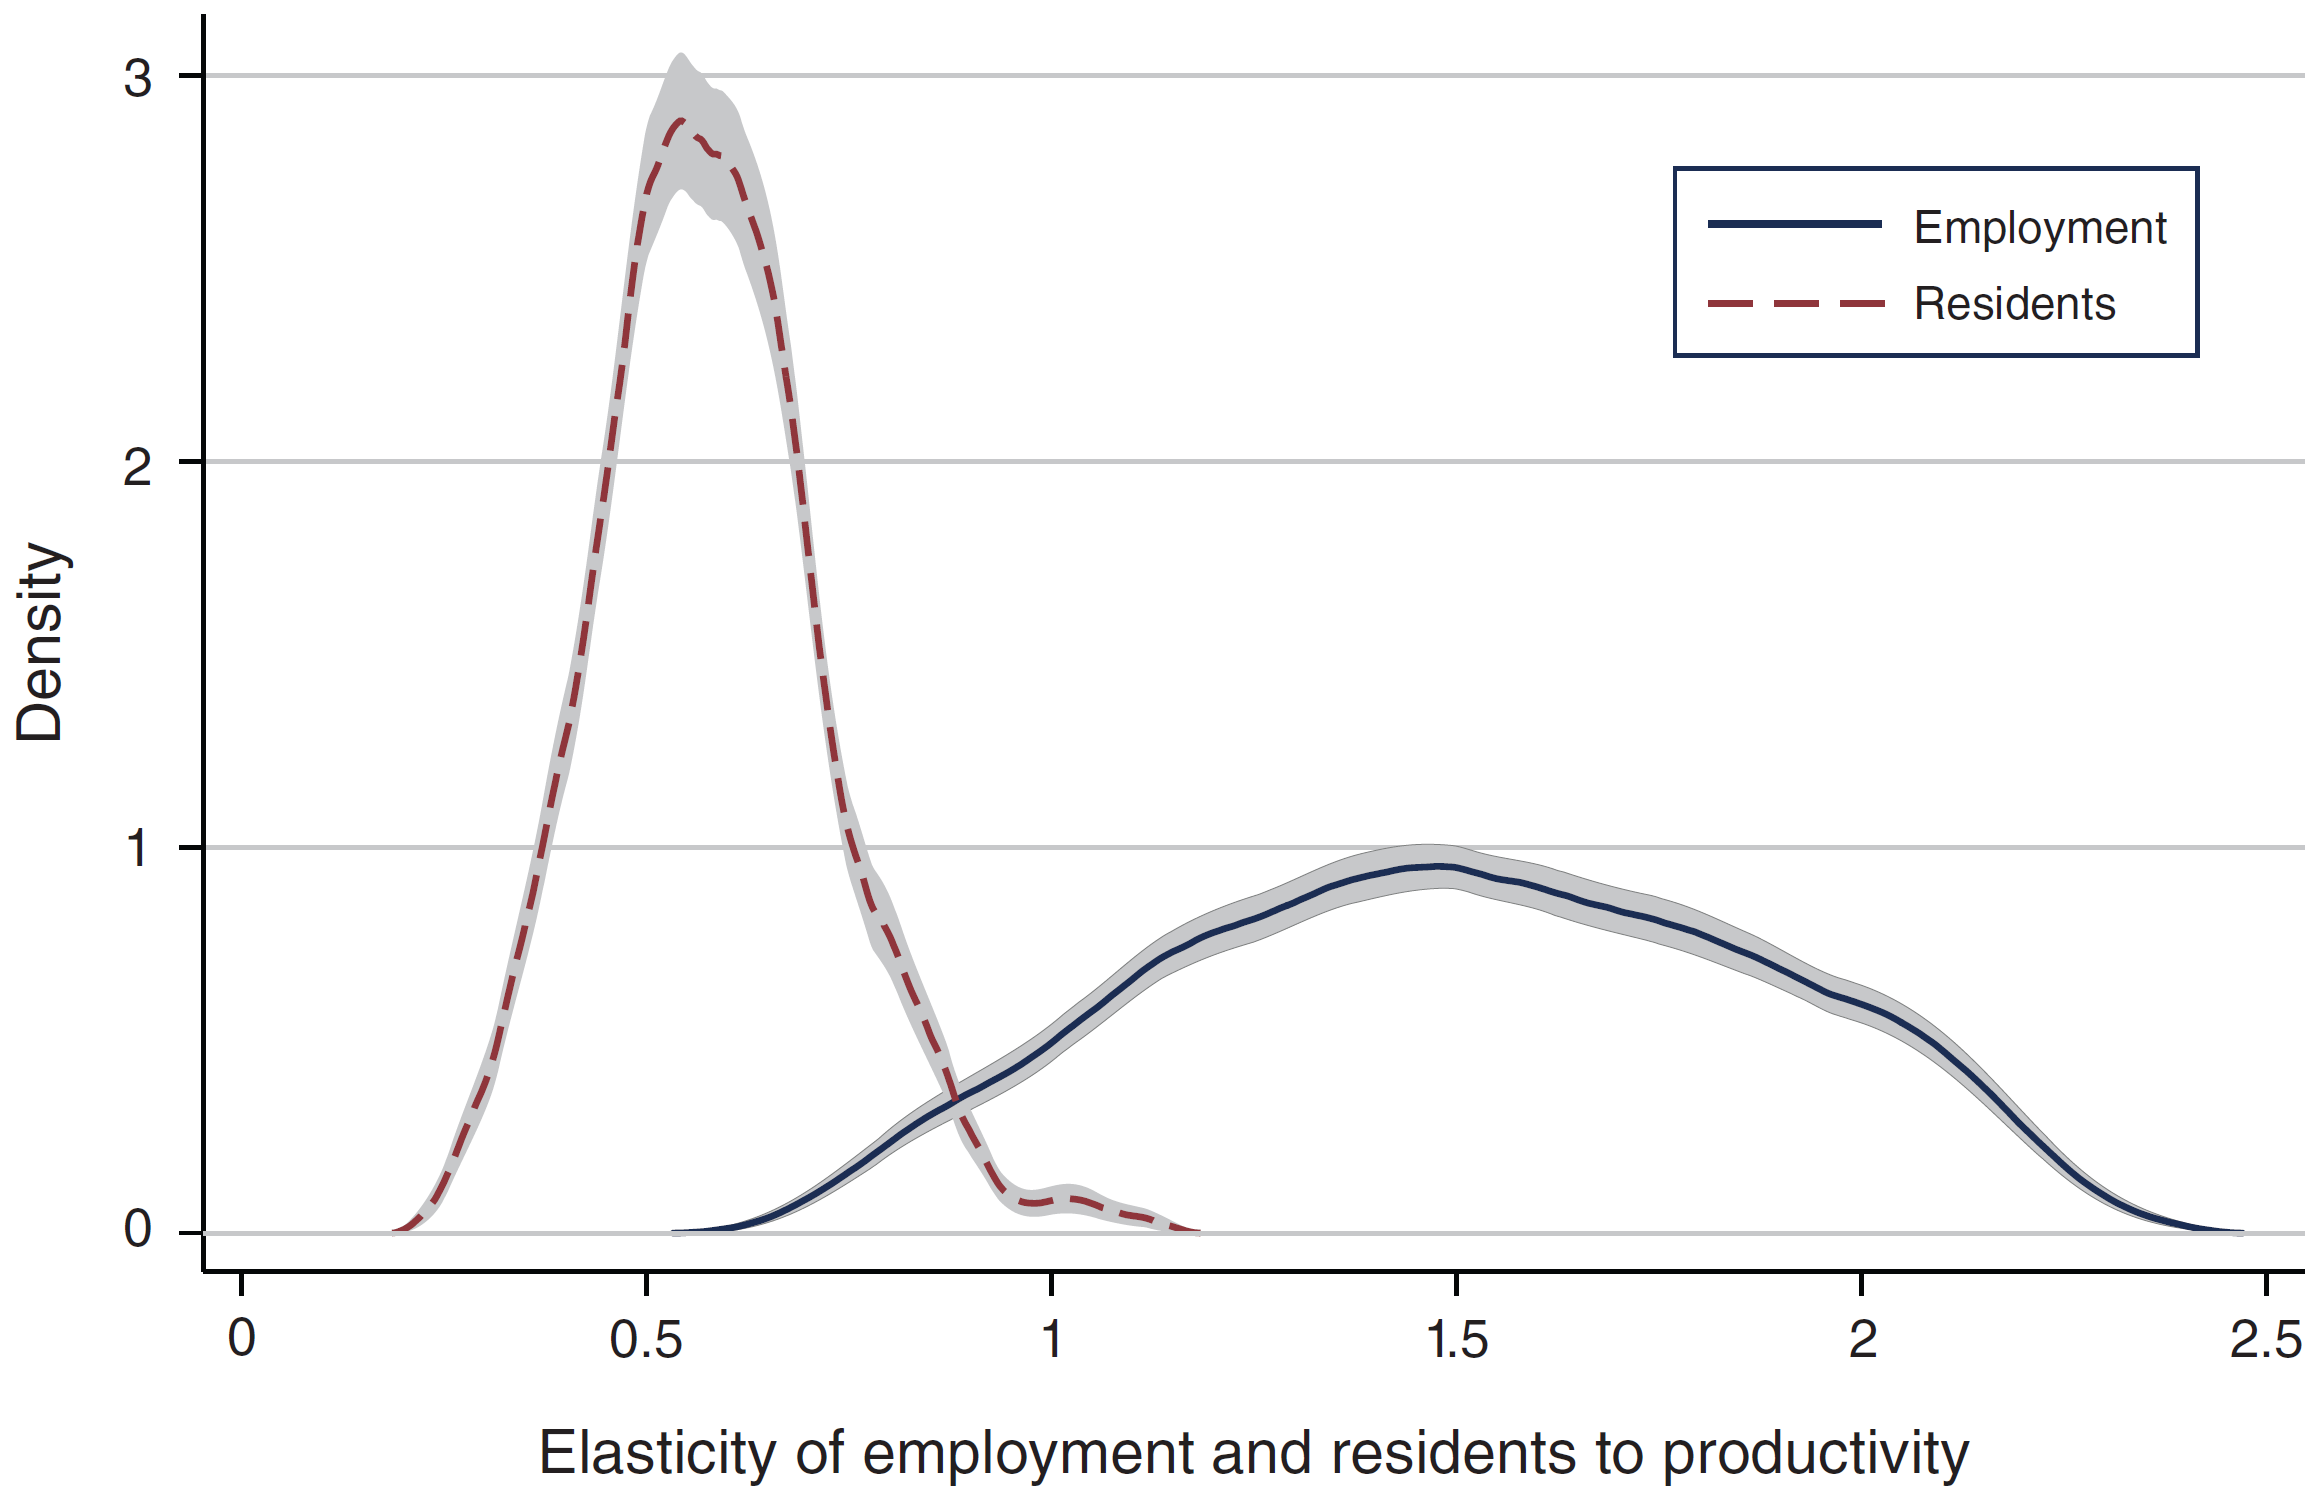
\includegraphics[width=0.8\textwidth]{fig2.png}
	\end{figure}
\end{frame}
%------------------------------------------------
\begin{frame}{Explain the GE local employment elasticities}
	The counterfactual exercises solve for the full GE effect of the productivity shock to each county.
	\medskip

	To provide intuition for the determinants of these local employment elasticities, we examine the relationship between these GE elasticities and a range of observed variables $\Rightarrow$
\end{frame}
%------------------------------------------------
\begin{frame}{Explain the GE local employment elasticities}
	\begin{figure}[htbp]
		\centering
		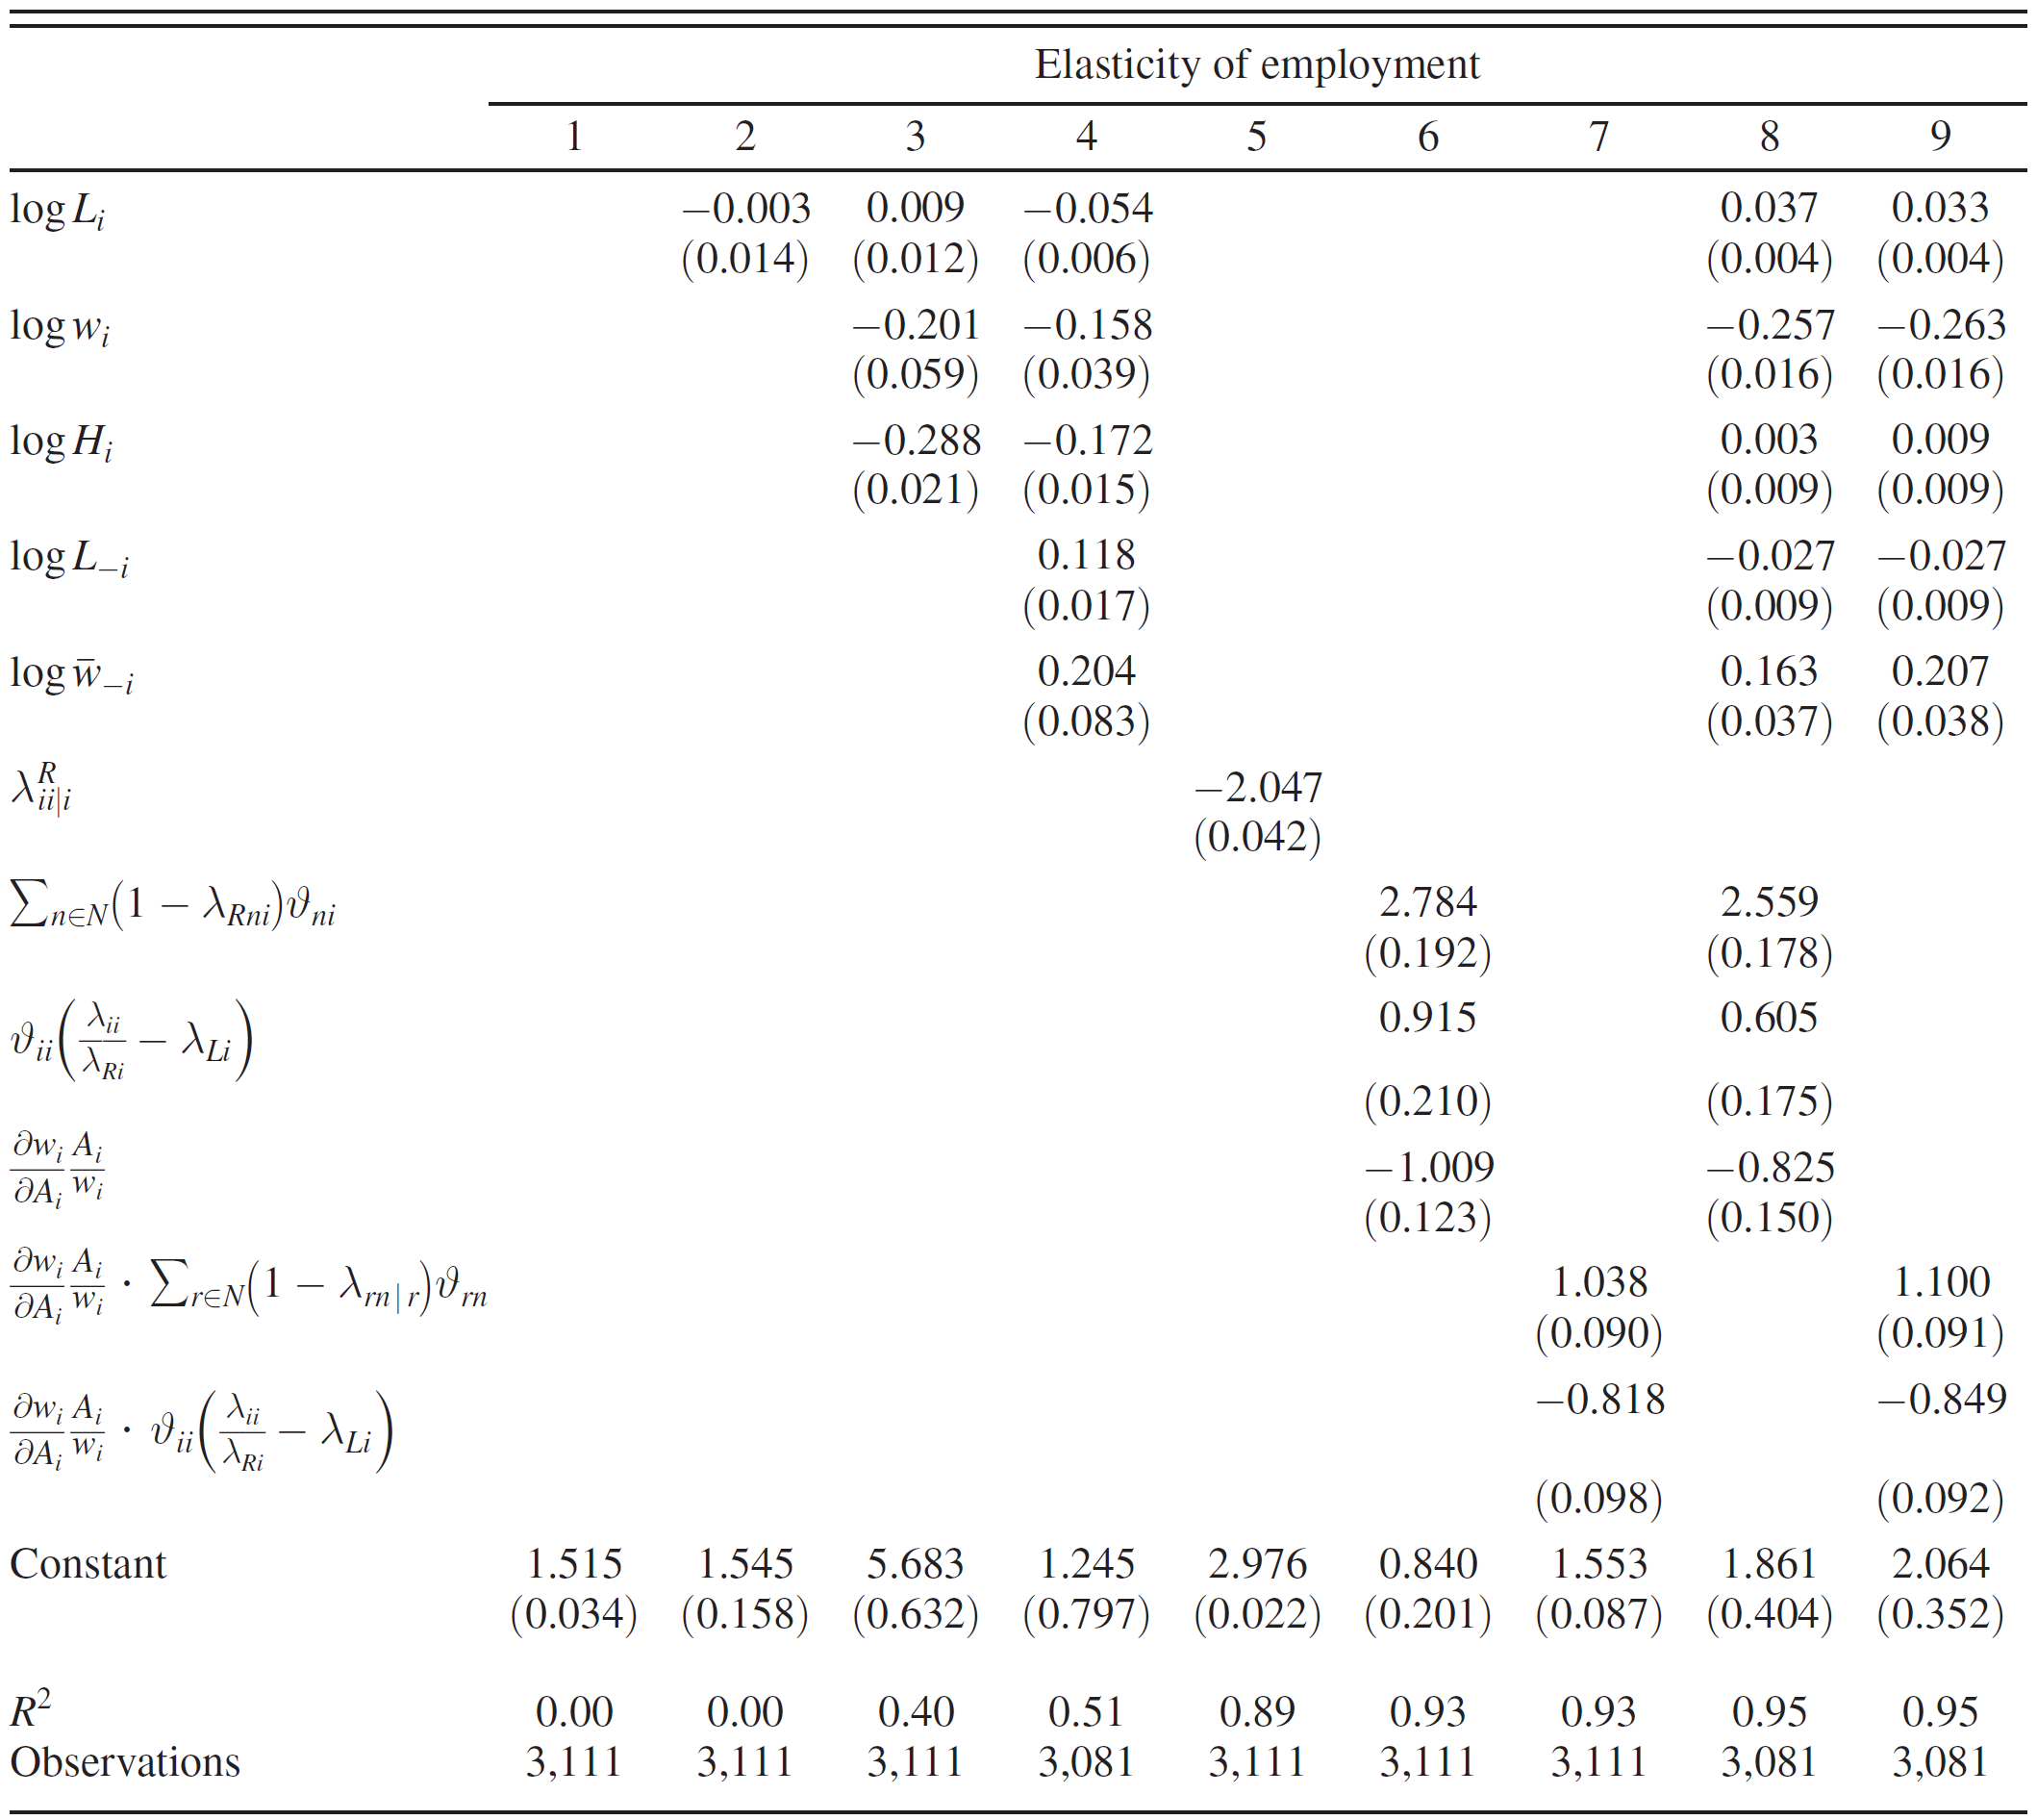
\includegraphics[width=0.69\textwidth]{tab2.png}		
	\end{figure}
\end{frame}
%------------------------------------------------
\begin{frame}{LATE of the productivity shock}
	We construct a regression sample including both treated and untreated counties from the 3111 counterfactuals ($3111^2=9678321$ observations).
	\medskip

	For each of these separate exercises, estimate a DID specification
	\begin{equation}
		\Delta \ln Y_{it} = a_0 + a_1I_{it} + a_2X_{it} + a_3\left(I_{it}\times X_{it}\right) + u_{it},
	\end{equation}
	where
	\begin{itemize}
		\item $i$ denotes the 3111 counties, $t$ indexes the 3111 counterfactuals;
		\item $\Delta \ln Y_{it}$ is the change in log employment between the counterfactual and actual equilibria;
		\item $I_{it}$ is a dummy for whether a county is shocked;
		\item $X_{it}$ are controls: model-suggested linkages measures v.s. more standard county controls.
	\end{itemize}
\end{frame}
%------------------------------------------------
\begin{frame}{A brief summary}
	\begin{itemize}
		\item The heterogeneity in PE elasticities is not well explained by standard county controls.
		\item In contrast, adding the measures of the openness to commuting, or the derived PE elasticities, can better explain this heterogeneity.
	\end{itemize}
	\medskip

	$\Rightarrow$ While capturing the full GE effects of productivity shocks requires solving the counterfactuals, augmenting DID regressions with commuting linkages captures in a reduced-form way the elasticity heterogeneity.
\end{frame}
%------------------------------------------------
\begin{frame}{Robustness: positive land supply elasticities}
	We now interpret the non-traded good as "developed" land and allow for a positive developed land supply elasticity that can differ across locations.
	\medskip
	\begin{block}{Assumption (Saiz, 2010)}
		The supply of land $H_n$ for each residence $n$ depends on the endogenous land price $Q_n$ as well as on the exogenous characteristics of locations $\bar{H}_n$.
		\medskip
		
		\textbf{Criterion:} Physical and regulatory constraints
	\end{block}
	\medskip
	$\Rightarrow$ When we undertake counterfactuals for productivity shocks, we focus on the subsample of counties within MSAs for which Saiz housing supply elasticities are available.
\end{frame}
%------------------------------------------------
\begin{frame}{Robustness: positive land supply elasticities}
	\begin{figure}[htbp]
		\centering
		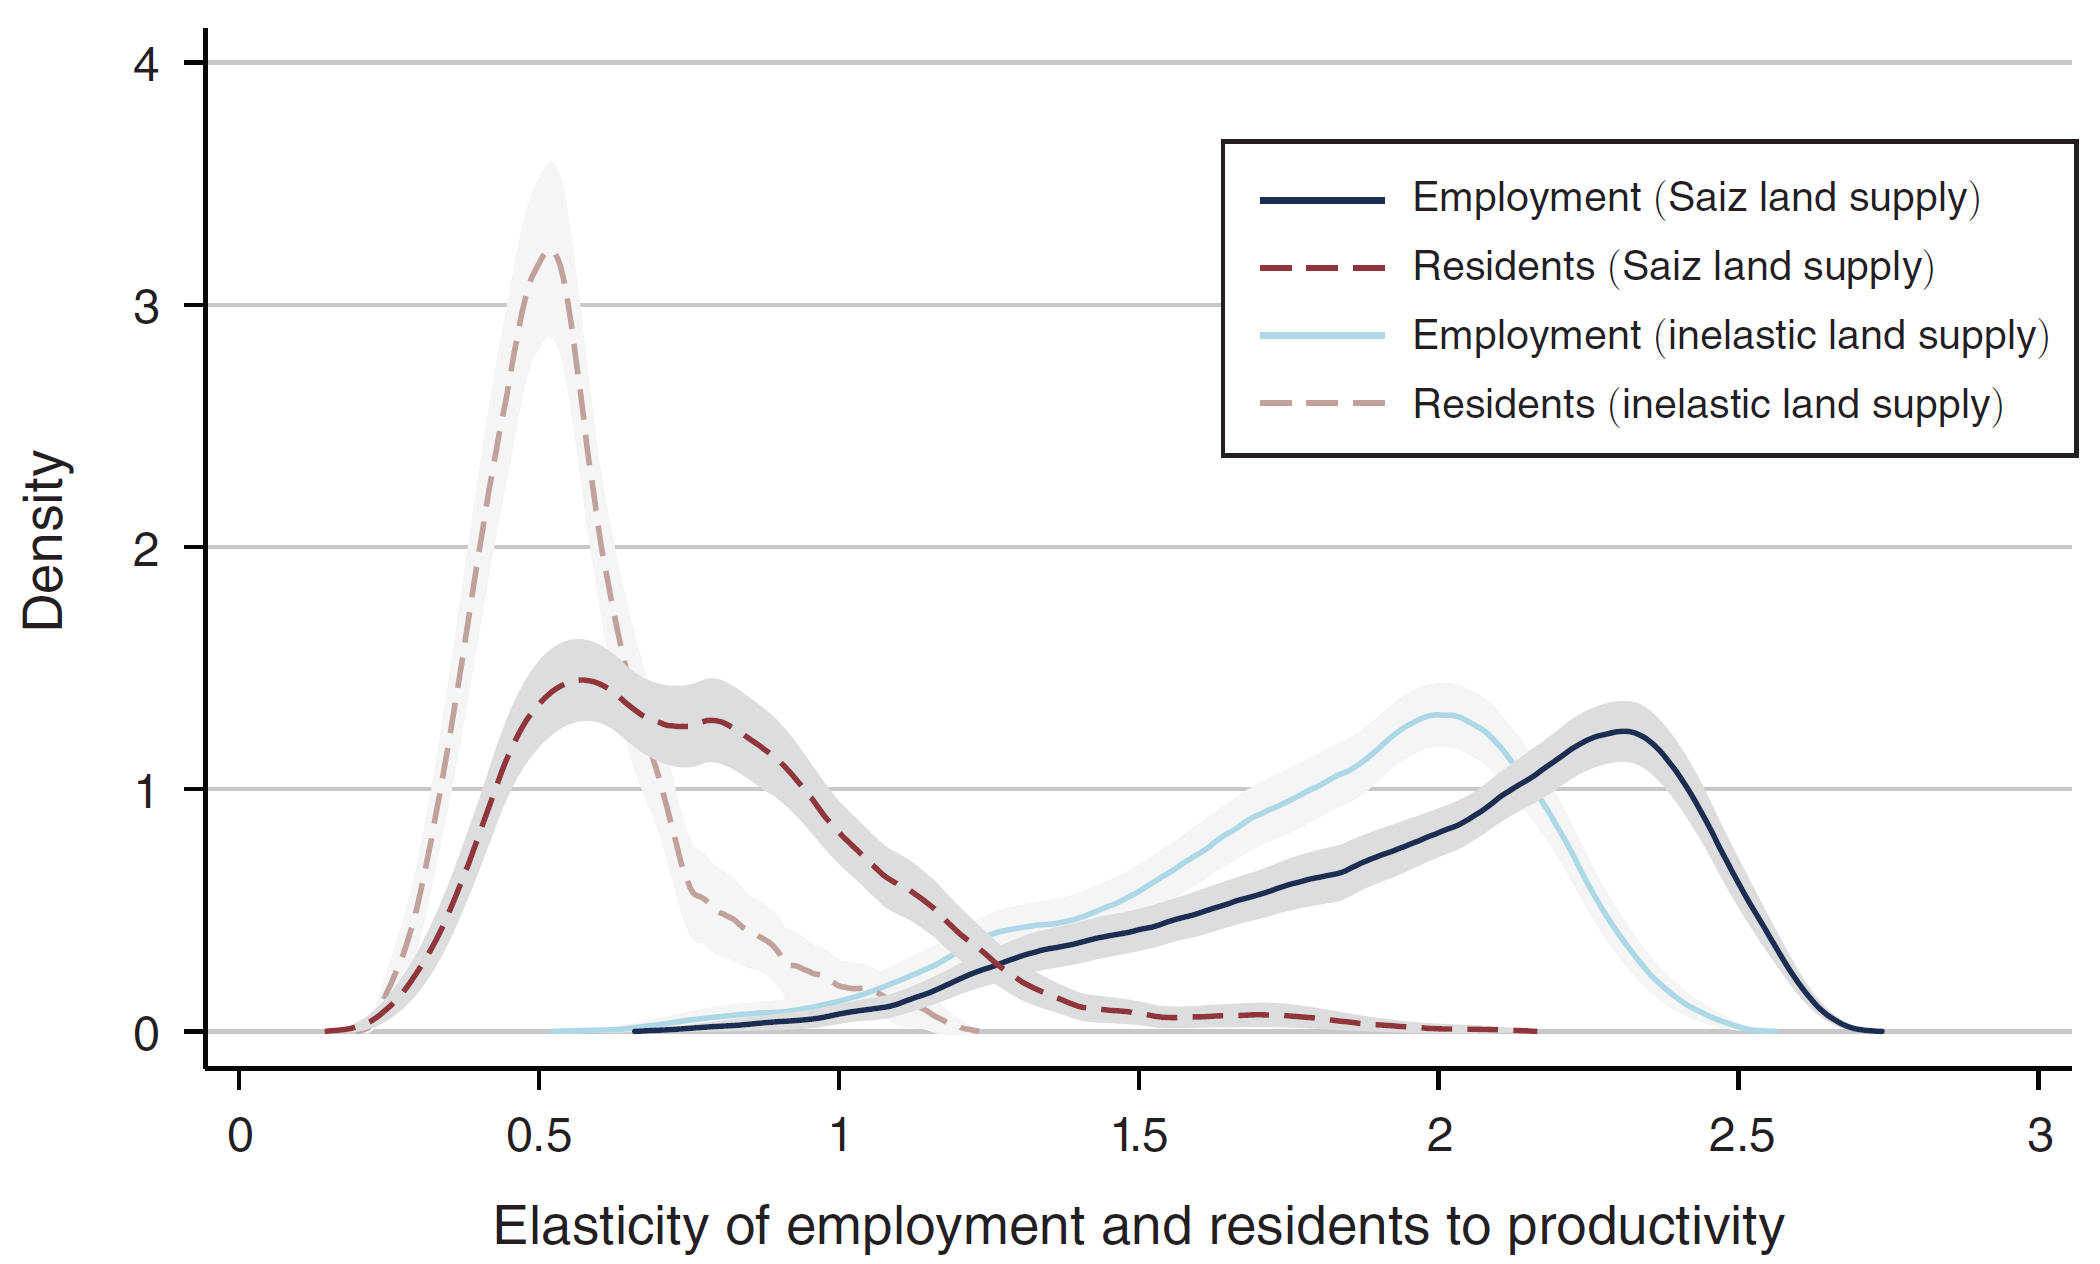
\includegraphics[width=0.9\textwidth]{fig3.png}
	\end{figure}
\end{frame}
%------------------------------------------------
\begin{frame}{Robustness: positive land supply elasticities}{Findings}
	Both distributions are shifted to the right.
	\begin{itemize}
		\item \textbf{Intuition:} The productivity shock induces an increase in the land supply, which relieves the rise in land prices and wages.
	\end{itemize}
	\medskip

	The heterogeneity in the elasticity of residents increases while the heterogeneity in the elasticity of employment changes little.
	\begin{itemize}
		\item \textbf{Intuition:} Commuting allows individuals to work in locations with inelastic housing supplies without living there. Therefore, housing supply elasticity impacts residence more than employment.
	\end{itemize}
	\begin{block}{}
		Improvement in commuting technologies is an alternative to relaxing land supply elasticities in enabling people to access high productivity locations.
	\end{block}
\end{frame}
%-------------------------------------------------------------------------
%-------------------------------------------------------------------------
\section{Million Dollar Plants}
\begin{frame}[shrink]
	\transfade %fade in and fade out
	\tableofcontents[sectionstyle=show/shaded,subsectionstyle=show/shaded/hide]
	\addtocounter{framenumber}{-1}
\end{frame}
%------------------------------------------------
\begin{frame}{Background}
	We provide separate empirical evidence for the importance of commuting in shaping the employment response to local labor demand shocks.
	\medskip

	\textbf{GHM setting}
	\begin{itemize}
		\item Use the location decisions of million dollar plants (MDP) as a source of variation in local labor demand.
		\item GHM use the revealed rankings of profit-maximizing firms.
		\item The losers are counties that narrowly lost the competition, which form a valid counterfactual for the winners.
	\end{itemize}
	\medskip

	\textbf{Data}
	\begin{itemize}
		\item The sample includes 166 winner and runner-up counties from 39 states from 1972 to 2003, where each case can have more than 2 counties (more than one runner up).
	\end{itemize}
\end{frame}
%------------------------------------------------
\begin{frame}{Replication of GHM (2010)}
	\begin{equation}
		\ln L_{it} = \kappa I_{j\tau} + \sum_{\tau=-10}^{10}\theta_\tau (T_\tau\times W_i) + \alpha_i + \eta_j + \mu_t + \varepsilon_{it}
	\end{equation}
	\begin{figure}[htbp]
		\centering
		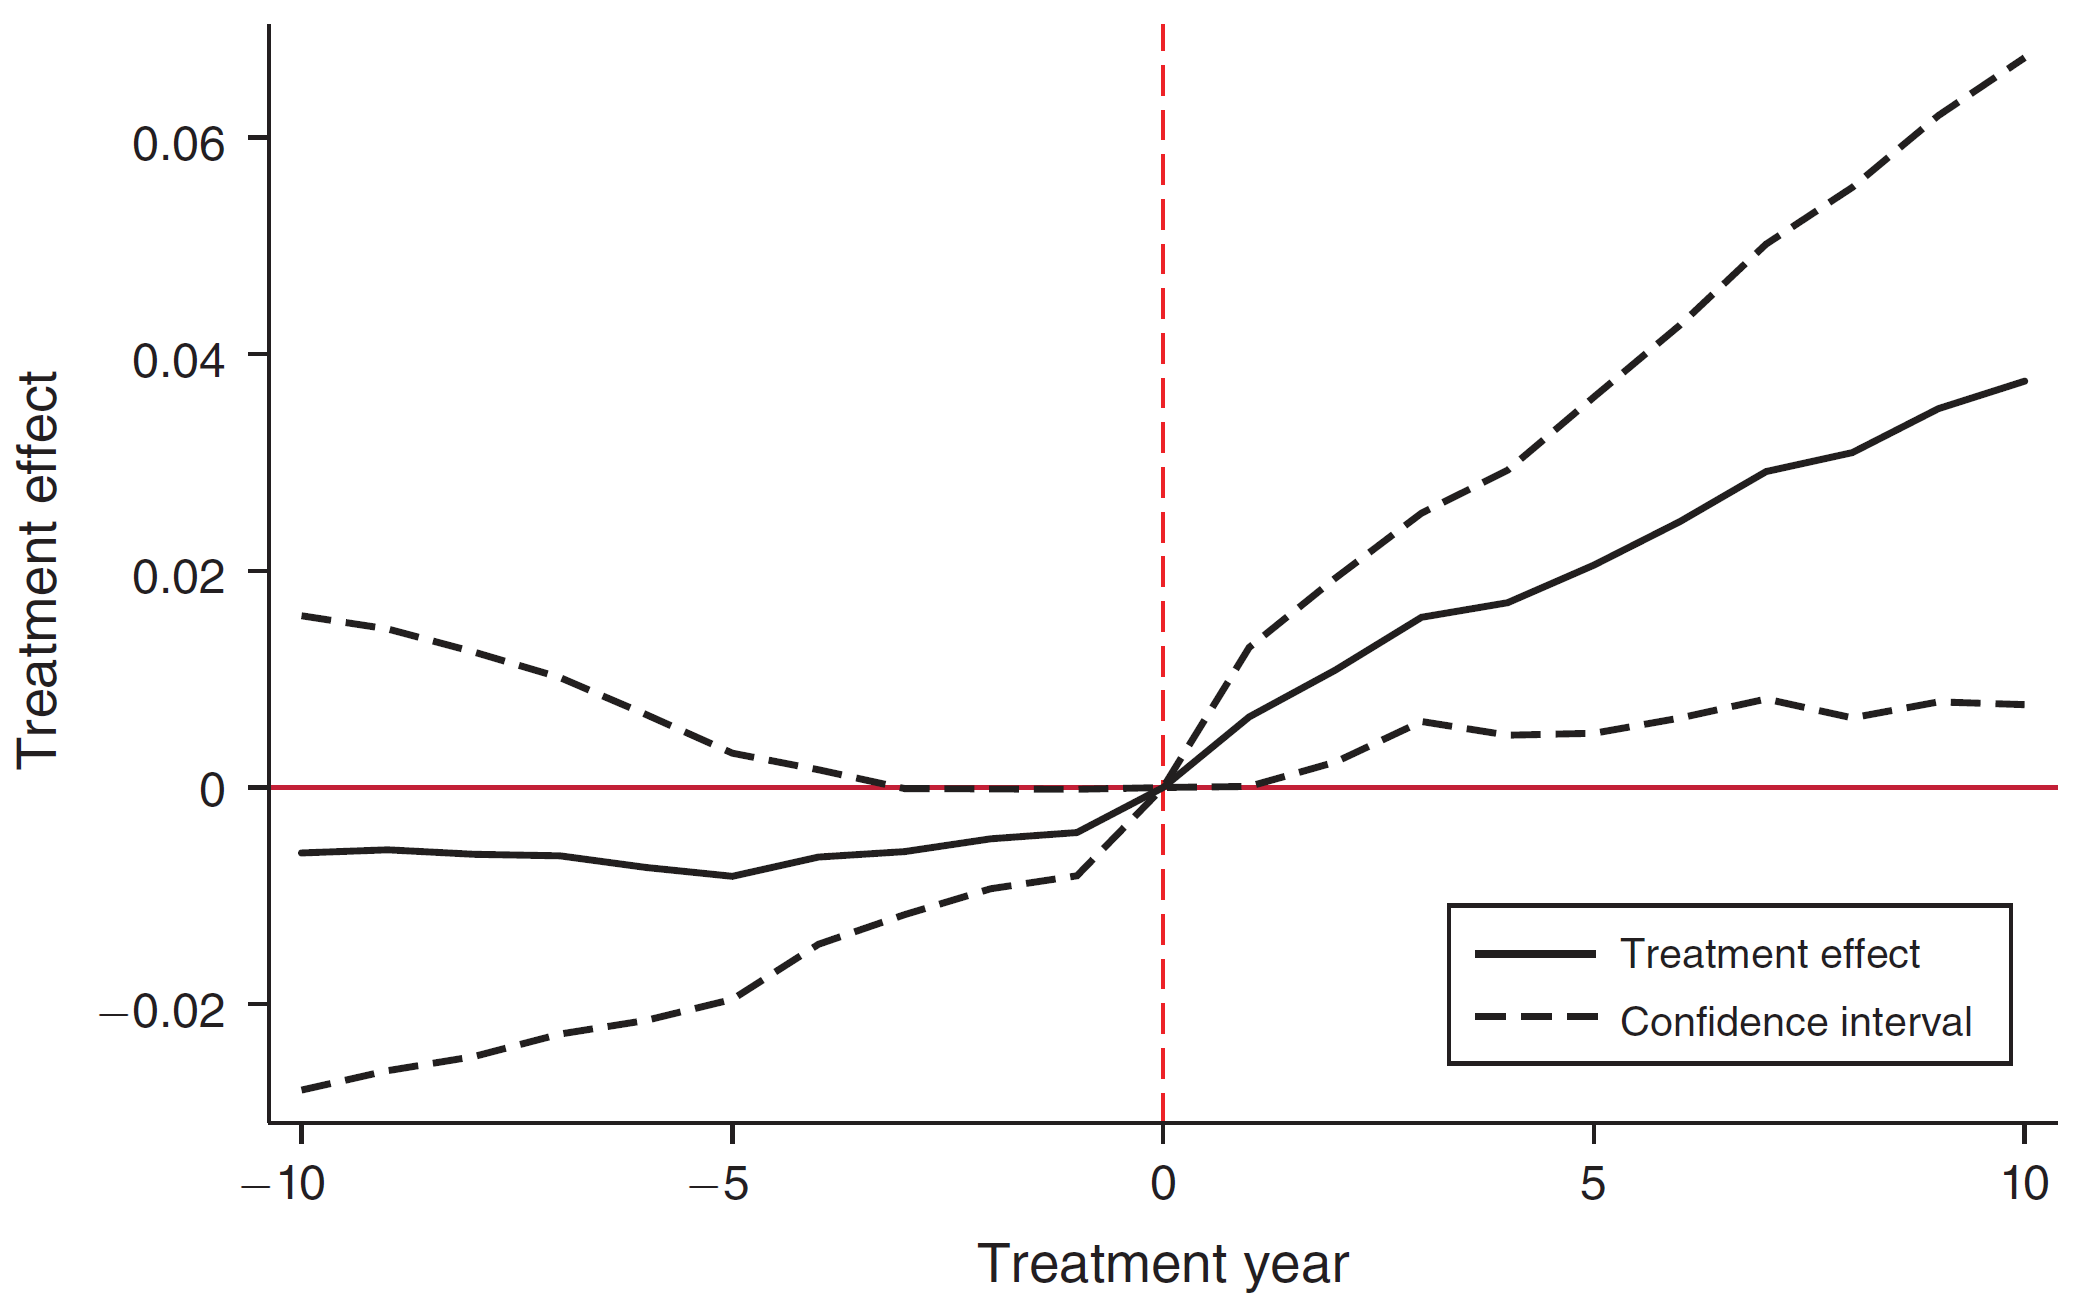
\includegraphics[width=0.8\textwidth]{fig4.png}
	\end{figure}
\end{frame}
%------------------------------------------------
\begin{frame}{Estimated MDP treatment and commuting openness}
	\begin{block}{Key prediction}
		The treatment effect of the MDP should be heterogeneous depending on openness to commuting.
	\end{block}
	\begin{equation}
		\begin{aligned}
			\ln L_{it} &= \kappa I_{j\tau} + \theta(I_{j\tau}\times W_i) + \beta(I_{j\tau}\times \lambda_{ii|i}^R) \\
			&+ \textcolor{red}{\gamma}(I_{j\tau}\times W_i\times \lambda_{ii|i}^R) + \alpha_i + \eta_j + \mu_t + \varepsilon_{it},
		\end{aligned}
	\end{equation}
	where
	\begin{itemize}
		\item $I_{j\tau}$ is an indicator for the treatment, which equals 1 for case $j$ from the treatment year onward and 0 otherwise,
		\item $W_i$ is an indicator for the winner county,
		\item $\lambda_{ii|i}^R$ is the residence own commuting share in 1990.
	\end{itemize}
\end{frame}
%------------------------------------------------
\begin{frame}{Estimated MDP treatment and commuting openness}
	\begin{figure}[htbp]
		\centering
		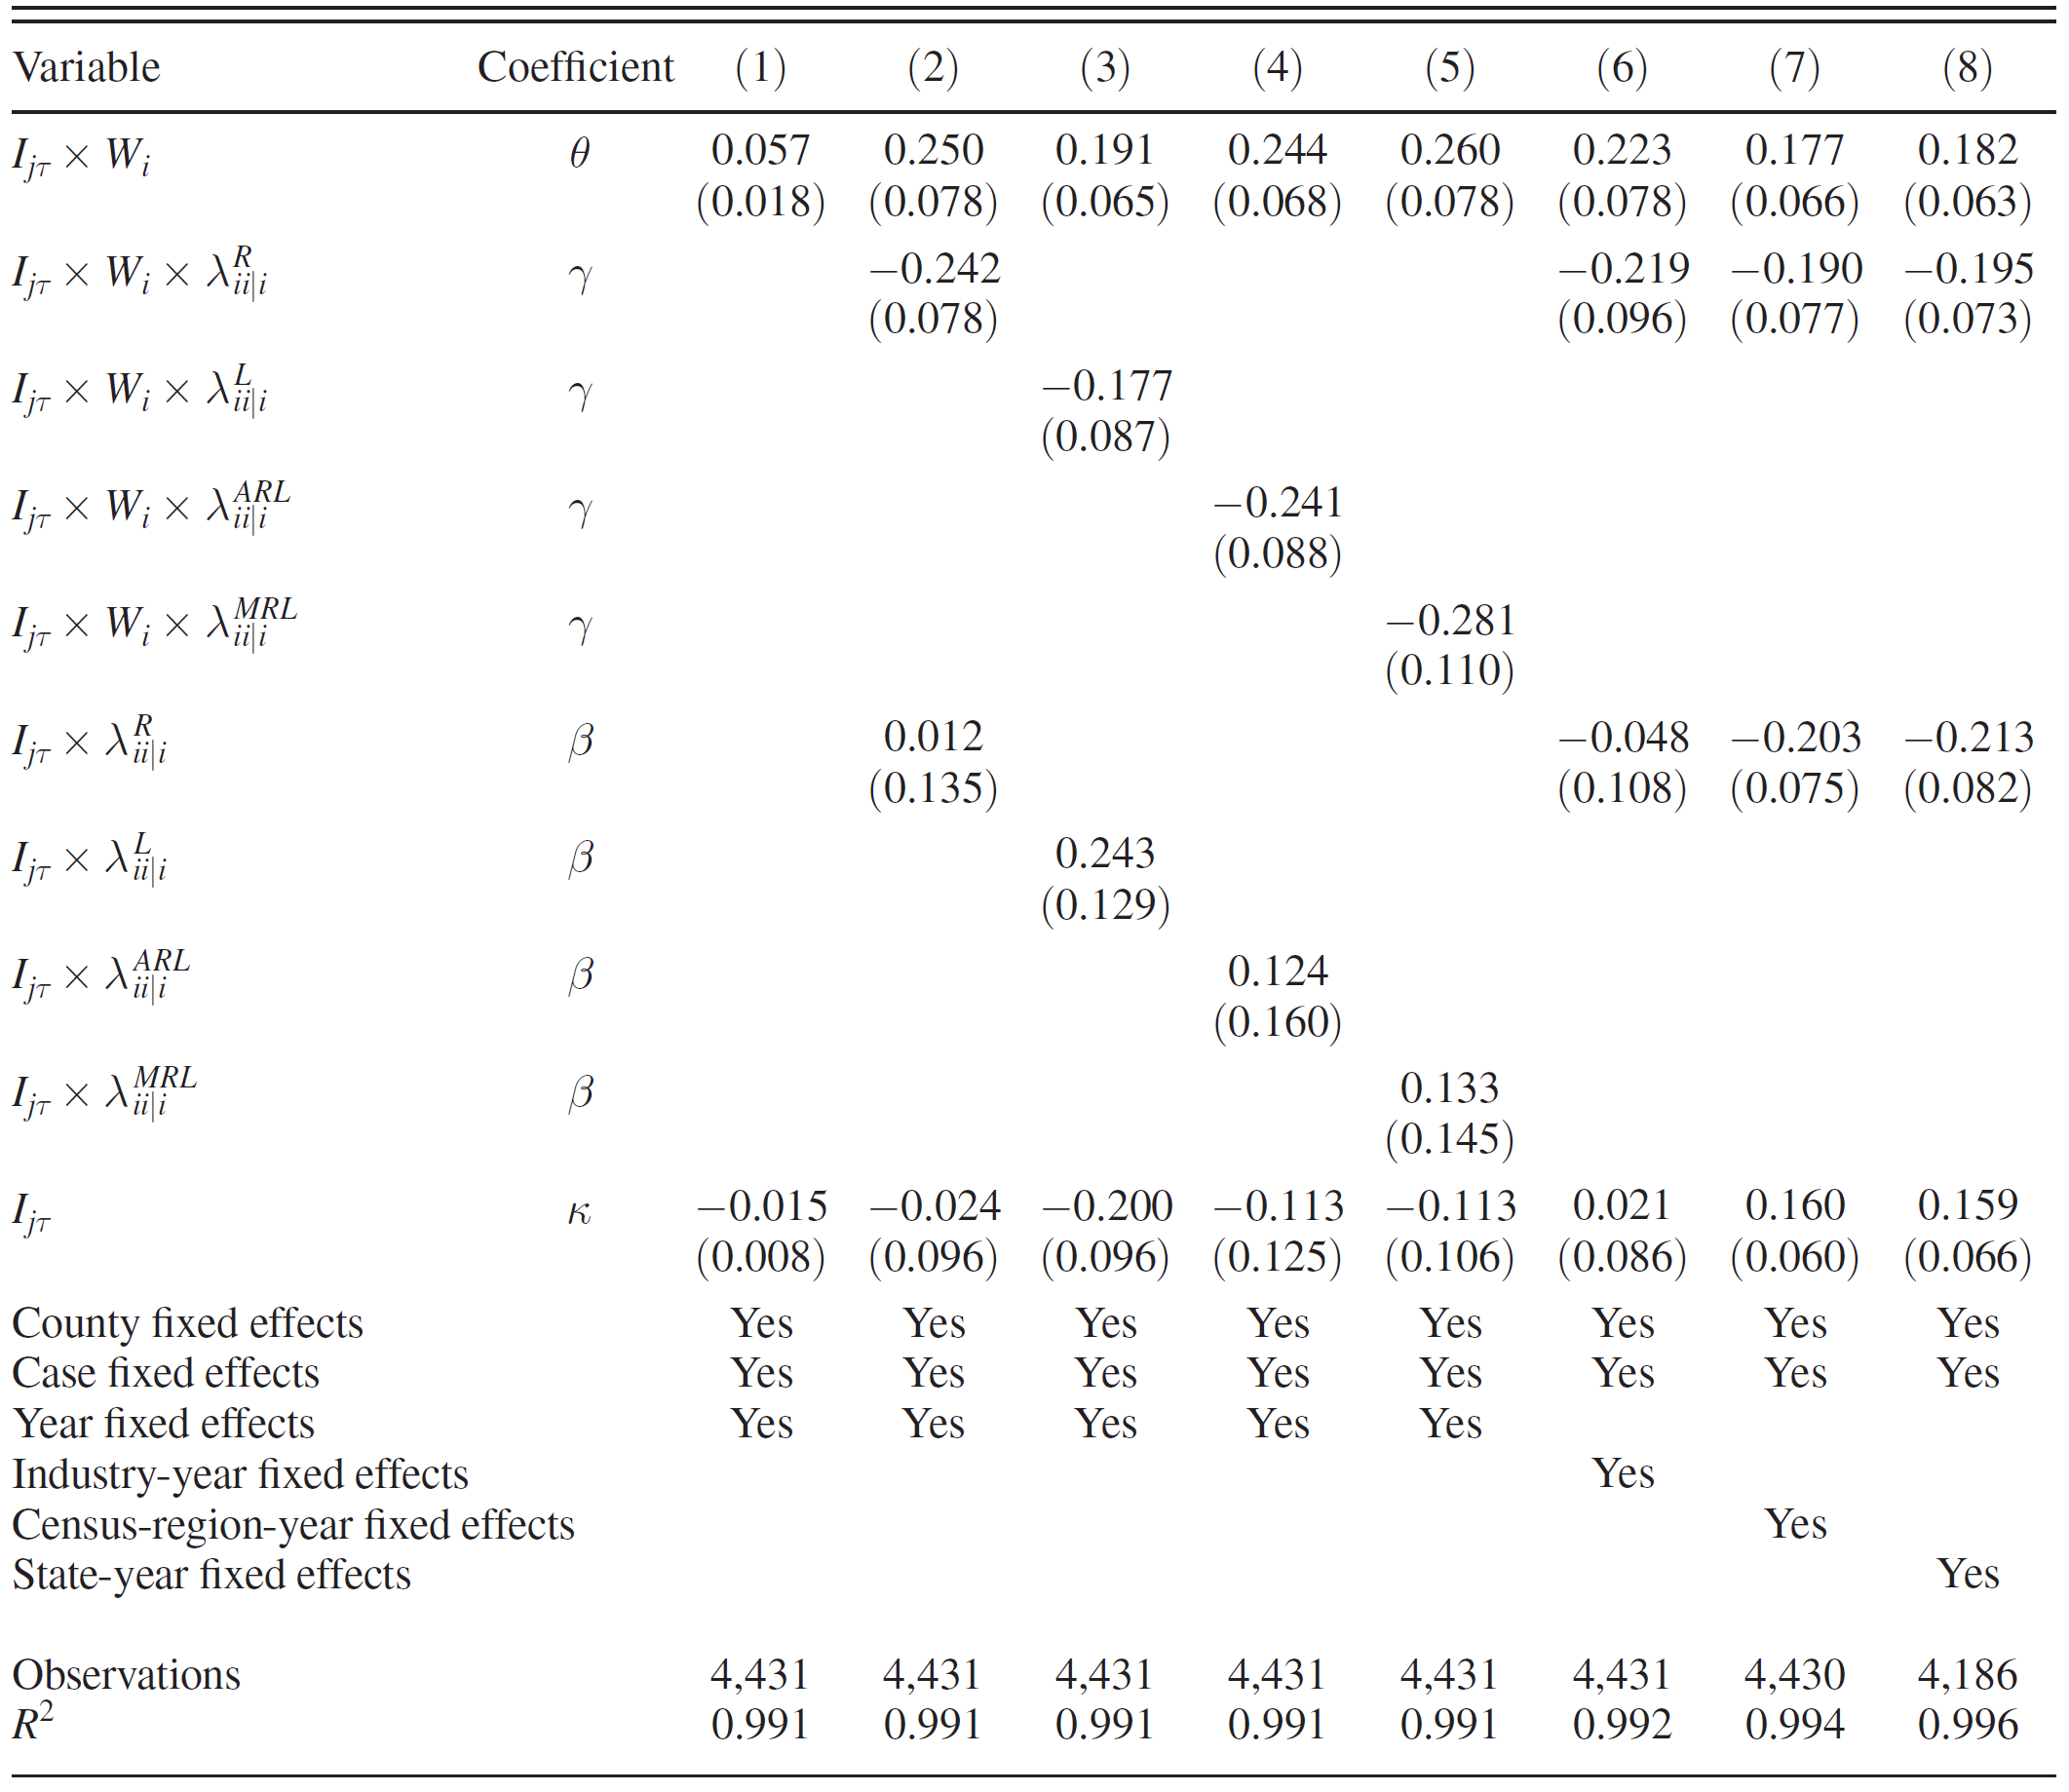
\includegraphics[width=0.7\textwidth]{tab3.png}
	\end{figure}
\end{frame}
%------------------------------------------------
\begin{frame}{Estimated MDP treatment and commuting openness}
	\textbf{Findings}
	\begin{itemize}
		\item $\gamma < 0$: the increases in employment is greater in response to the positive labor demand shock in counties with more open local labor markets (lower $\lambda_{ii|i}^R$).
		\item The opening of a MDP has little effect on employment in counties that are completely closed to commuting ($\lambda_{ii|i}\to 1 \Rightarrow \theta+\gamma\approx 0$).
		\item The increase in employment in the treated counties comes at the expense of reduced employment in neighboring counties.
	\end{itemize}
\end{frame}
%------------------------------------------------
\begin{frame}{Check for pre-trend}
	\begin{small}
		\begin{equation}
			\begin{aligned}
				\ln L_{it} &= \kappa I_{j\tau} + \sum_{\tau=-10}^{10}\theta_{\tau}(T_{\tau}\times W_i) + \sum_{\tau=-10}^{10}\beta_\tau(T_{\tau}\times \lambda_{ii|i}^R) \\
				&+ \sum_{\tau=-10}^{10}\gamma_\tau(T_{\tau}\times W_i\times \lambda_{ii|i}^R) + \alpha_i + \eta_j + \mu_{st} + \varepsilon_{it}
			\end{aligned}
		\end{equation}
	\end{small}
	\begin{figure}[htbp]
		\centering
		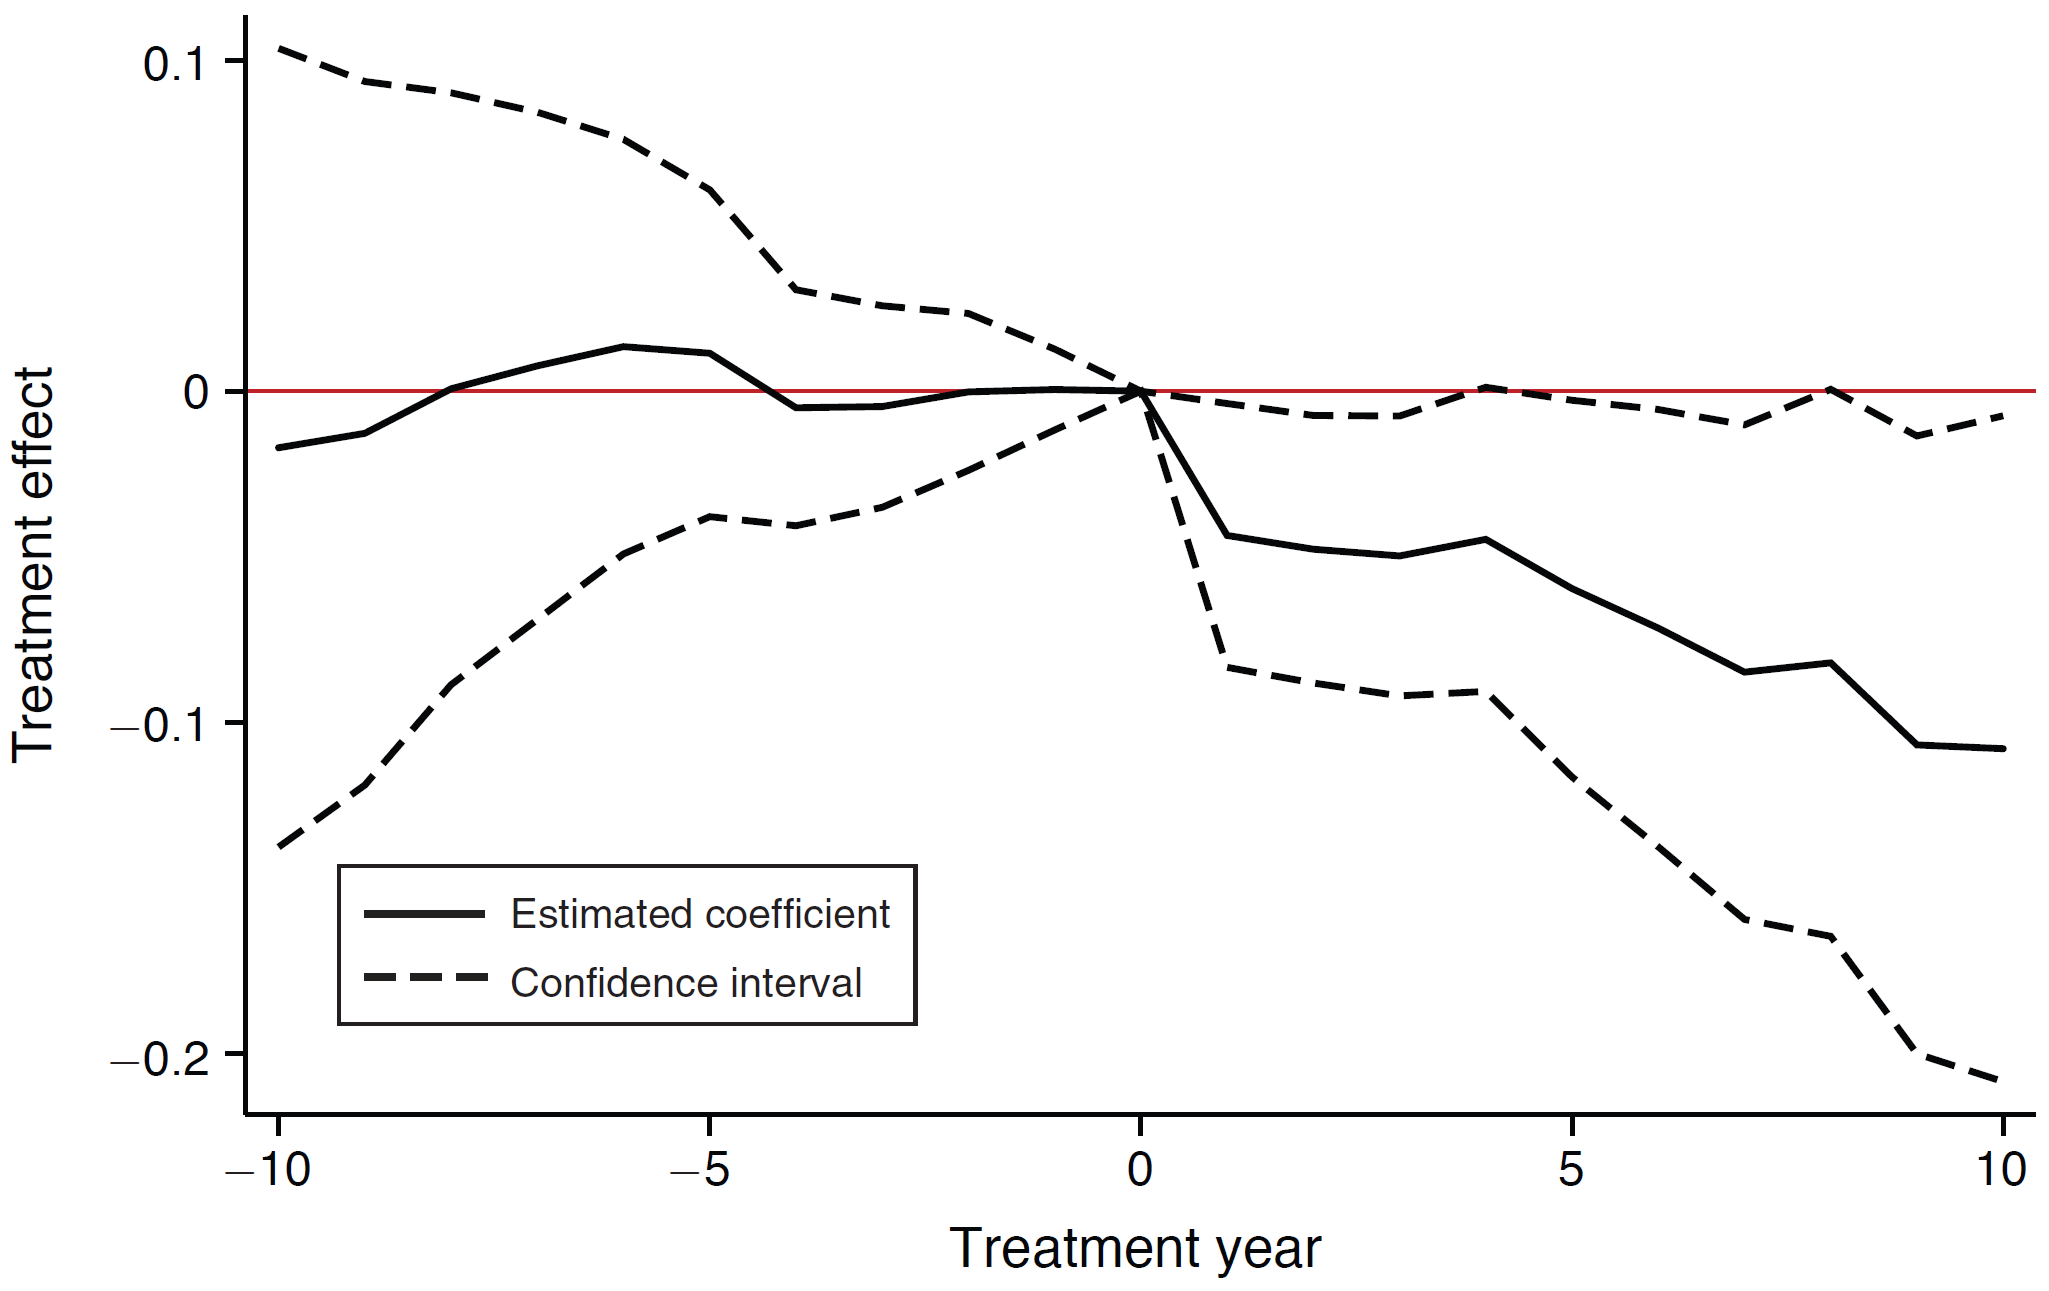
\includegraphics[width=0.66\textwidth]{fig5.png}
	\end{figure}
\end{frame}
%------------------------------------------------
\begin{frame}{Nonparametric specification}
	\begin{equation}
		\ln L_{it} = \kappa I_{j\tau} + \sum_{j=1}^{J}\textcolor{red}{\theta_j}(I_{j\tau}\times W_i) + \alpha_i + \eta_j + \mu_{t} + \varepsilon_{it}
	\end{equation}
	where $\theta_j$ captures the relative increase in employment in the winner county in case $j$ following the MDP announcement.
	\begin{figure}[htbp]
		\centering
		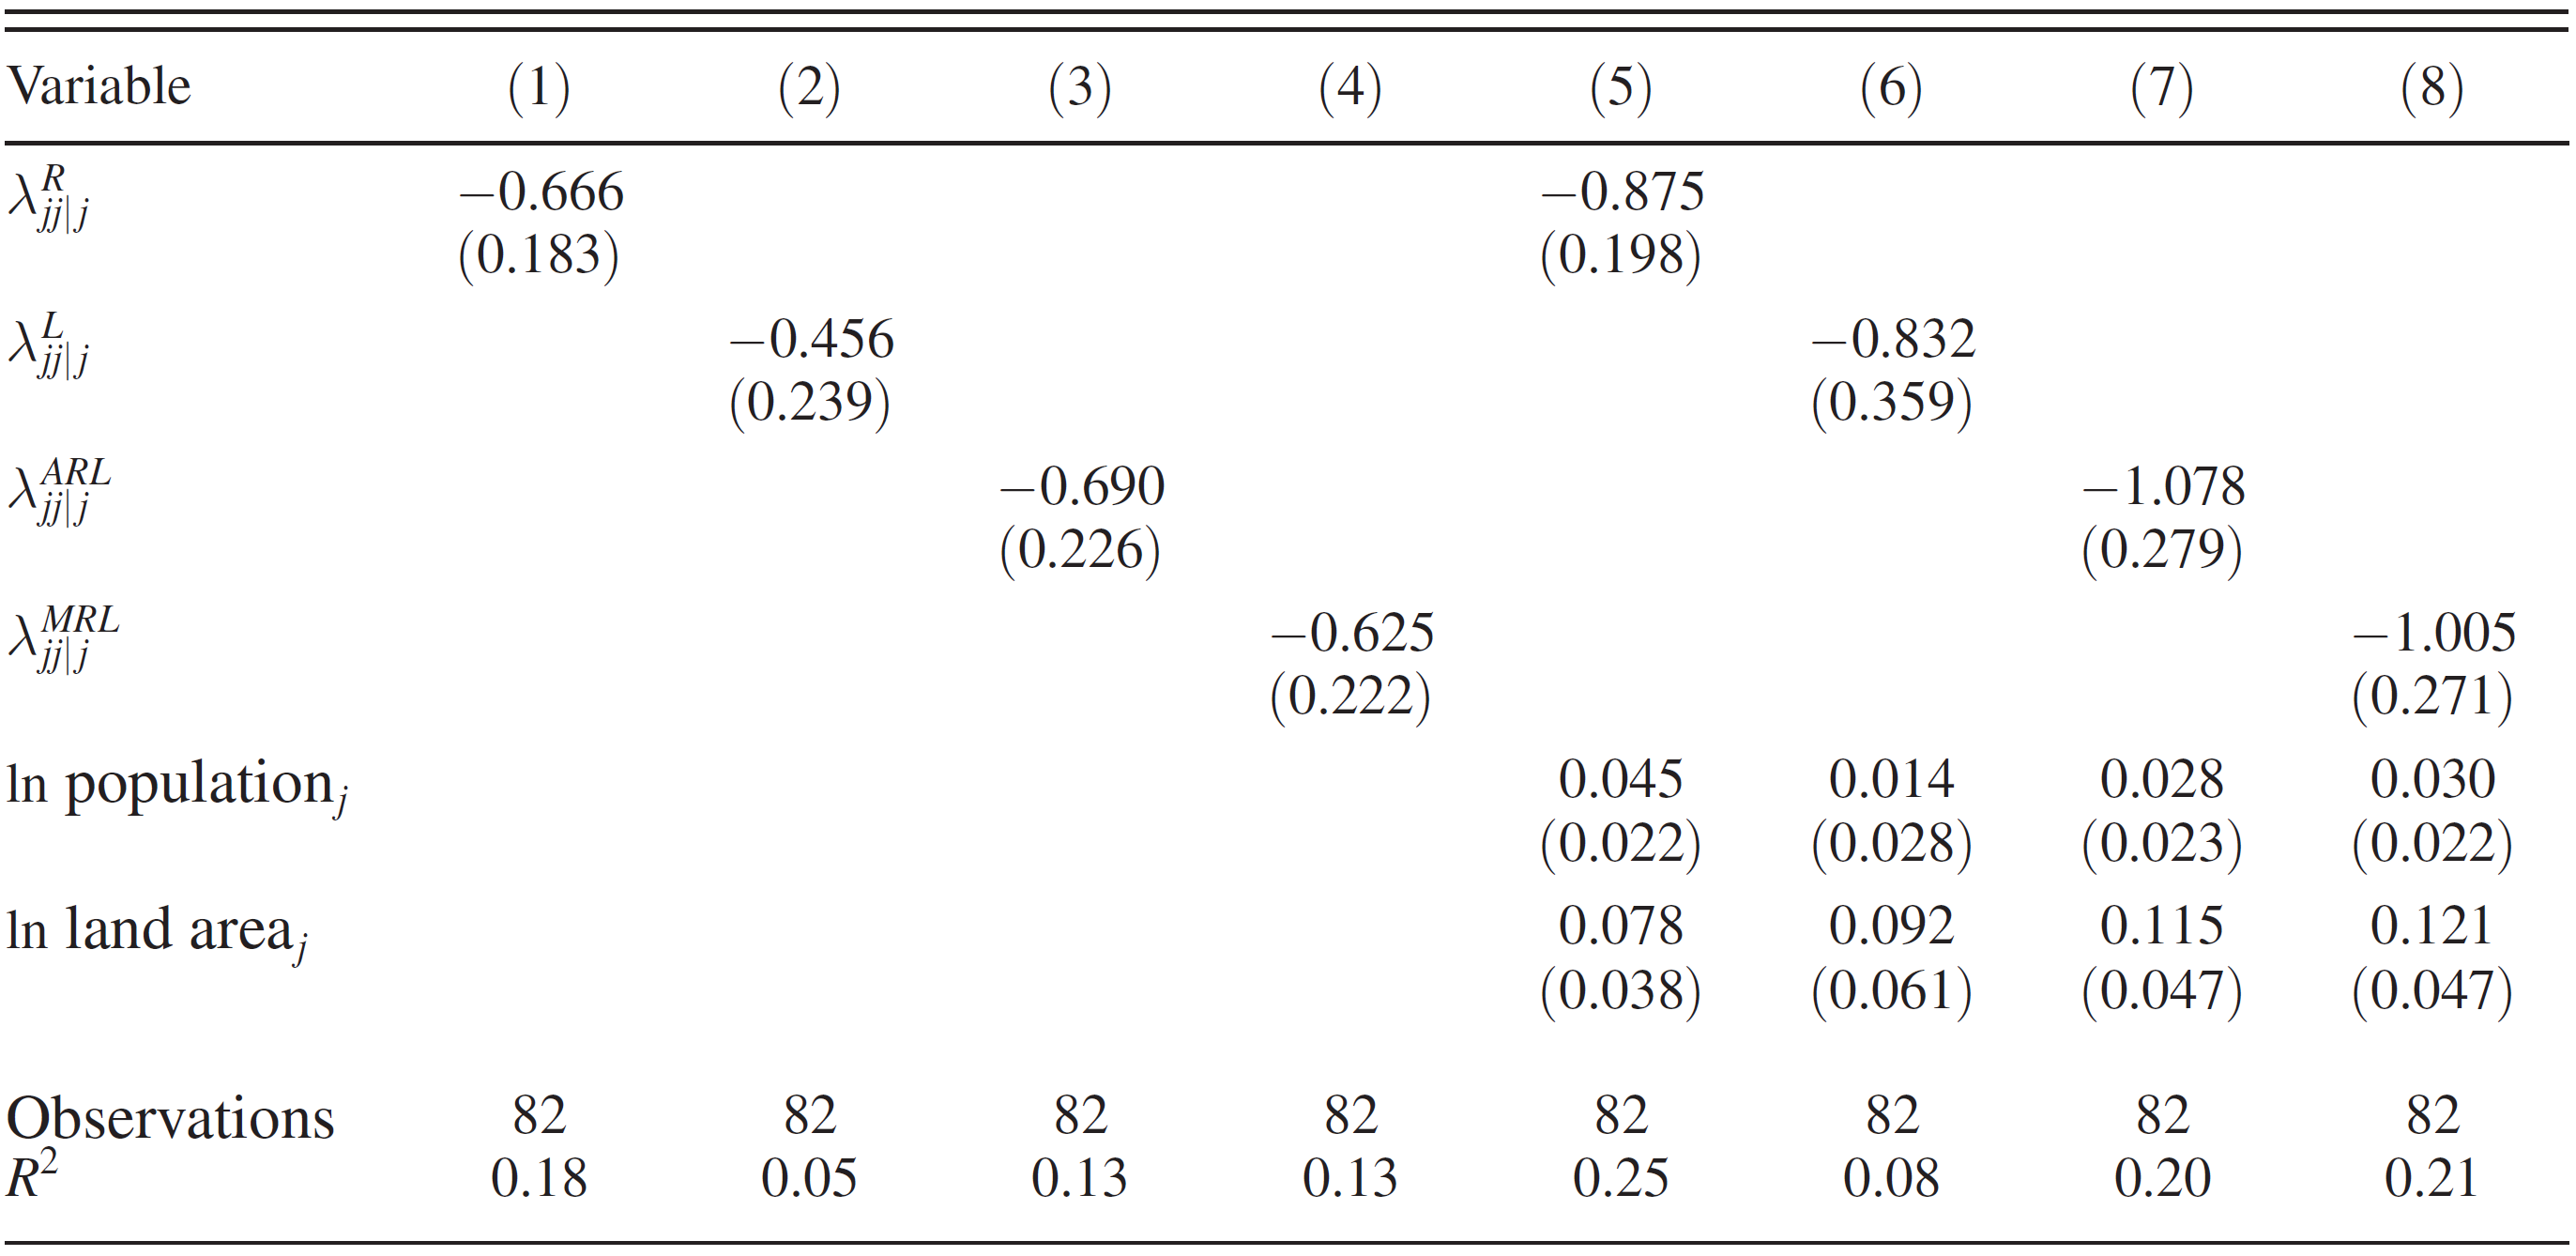
\includegraphics[width=0.8\textwidth]{tab4.png}
	\end{figure}
\end{frame}
%-------------------------------------------------------------------------
%-------------------------------------------------------------------------
\section{Changes in Commuting Costs}
\begin{frame}[shrink]
	\transfade %fade in and fade out
	\tableofcontents[sectionstyle=show/shaded,subsectionstyle=show/shaded/hide]
	\addtocounter{framenumber}{-1}
\end{frame}
%------------------------------------------------
\begin{frame}{Changes in commuting costs}
	Commuting linkages also matter for the aggregate spatial distribution of economic activity and welfare.
	\medskip

	\textbf{Setting:} We use the observed commuting data to back out implied values of $\mathcal{B}_{ni}$ $(\;\equiv B_{ni}\kappa_{ni}^\epsilon\;)$ capturing the ease of commuting.
	\begin{equation}
		\tilde{\mathcal{B}}_{ni} \equiv \left(\frac{\mathcal{B}_{ni}\mathcal{B}_{in}}{\mathcal{B}_{nn}\mathcal{B}_{ii}}\right)^{1/2} = \left(\frac{L_{ni}L_{in}}{L_{nn}L_{ii}}\right)^{1/2}.
	\end{equation}
	\medskip

	We compute with data in 1990 and 2010, and calculate the change rate:
	\begin{table}[]
		\begin{tabular}{cc}
		\hline \hline
		$\hat{\tilde{\mathcal{B}}}_{ni}$    & Percentile  \\ \hline
		0.96 & 25\% \\
		0.88 & 50\% \\
		0.79 & 75\% \\ \hline
		\end{tabular}
	\end{table}
\end{frame}
%------------------------------------------------
\begin{frame}{Welfare implications}
	We assume a common reduction or increase in the costs of commuting for all counties equal to percentiles of this distribution $\{\hat{\tilde{\mathcal{B}}}_{ni}\}$.
	\medskip

	The welfare change from the shock to commuting costs can be decomposed as follows:
	\begin{equation}
		\hat{\bar{U}} = \left(\frac{1}{\hat{\lambda}_{ii}} \right)^{1/\epsilon}\left(\frac{1}{\hat{\pi}_{ii}}\right)^{\frac{\alpha}{\sigma-1}}\left(\frac{\hat{w}_i}{\hat{\bar{v}}_i}\right)^{1-\alpha}\frac{\hat{L}_i^{\frac{\alpha}{\sigma-1}}}{\hat{R}_i^{1-\alpha}}.
	\end{equation}
	\begin{figure}[htbp]
		\centering
		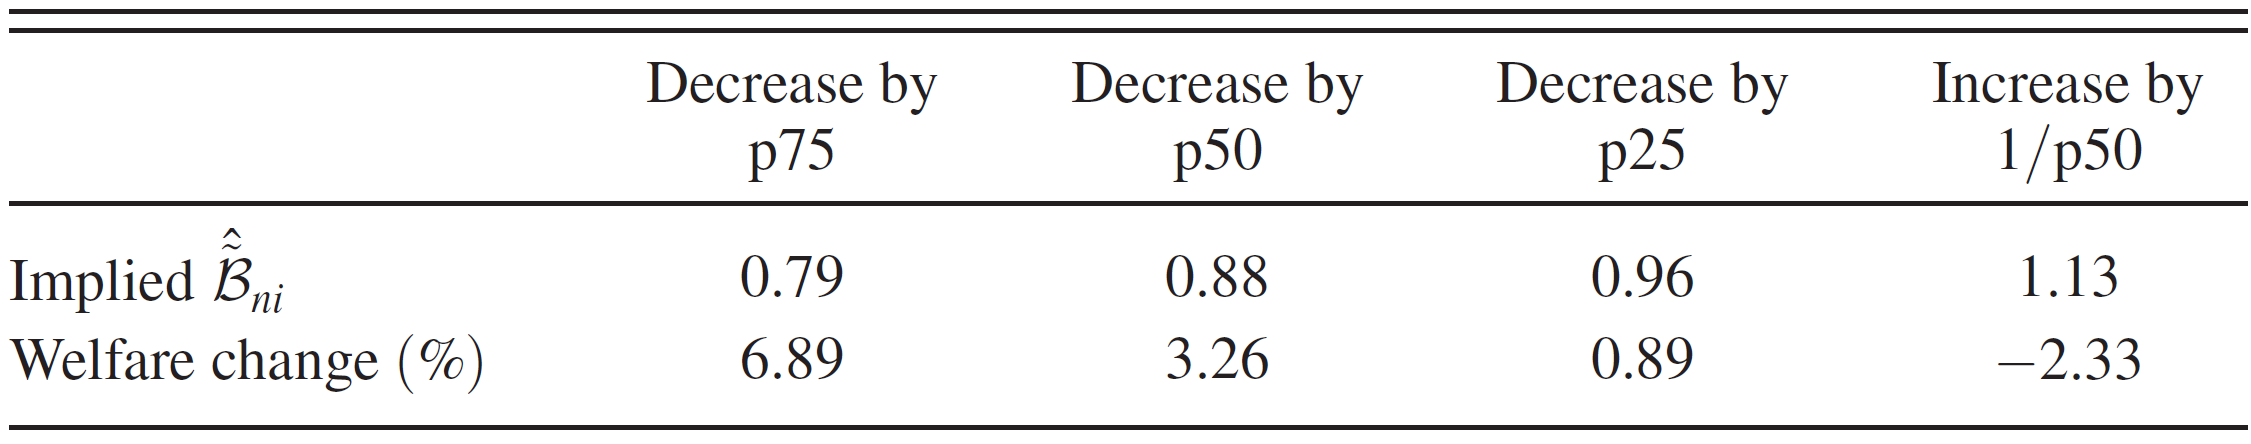
\includegraphics[width=0.9\textwidth]{tab5.png}
	\end{figure}
\end{frame}
%-------------------------------------------------------------------------
%-------------------------------------------------------------------------
\section{Conclusion}
\begin{frame}[shrink]
	\transfade %fade in and fade out
	\tableofcontents[sectionstyle=show/shaded,subsectionstyle=show/shaded/hide]
	\addtocounter{framenumber}{-1}
\end{frame}
%------------------------------------------------
\begin{frame}{Conclusion}
	\begin{itemize}
		\item We develop a quantitative spatial GE model that incorporates spatial linkages between locations in both goods markets and factor markets.
		\item We find substantial heterogeneity across both counties and CZs in the elasticity of local employment to a productivity shock.
		\item The quasi-experiment shows larger increases in employment in response to labor demand shocks in counties with more open commuting markets, consistent with the predictions of our model.
		\item Commuting also matters in the aggregate for the spatial distribution of economic activity and welfare.
	\end{itemize}
\end{frame}
%------------------------------------------------
%------------------------------------------------
\begin{frame}
	\Huge{\centerline{\textit{The End}}}
\end{frame}
%-------------------------------------------------------------------------

\end{document} 